\documentclass[a4paper, twoside, 10pt]{report}

%% Language and font encodings
\usepackage[english]{babel}
\usepackage[utf8]{inputenc}
\usepackage[T1]{fontenc}

%% Sets page size and margins
\usepackage[a4paper,top=3cm,bottom=2cm,left=3cm,right=3cm,marginparwidth=1.75cm]{geometry}

%% Useful packages
\usepackage[backend=biber,style=imperialharvard]{biblatex}
\usepackage{afterpage}
\usepackage{amsmath}
\usepackage{amsthm}
\usepackage{csquotes}
\usepackage{enumitem}
\usepackage{graphicx}
\usepackage{lipsum}
\usepackage{booktabs}

\usepackage{titlesec}

\usepackage{amssymb}
\usepackage{multirow}

\usepackage{subcaption}
\usepackage{blindtext}
\usepackage{quotchap}
\usepackage{makecell}

\usepackage{wrapfig}
\usepackage{float}


% Listings (for displaying code):
\usepackage{listings}
\lstset{
    frame = single, 
    framexleftmargin=15pt
}

% Center figure captions:
\usepackage[labelfont=bf,justification=centering]{caption}

% ----------- Algorithm2e setup
\usepackage[ruled,vlined]{algorithm2e}
\makeatletter
\renewcommand{\SetKwInOut}[2]{%
  \sbox\algocf@inoutbox{\KwSty{#2}\algocf@typo:}%
  \expandafter\ifx\csname InOutSizeDefined\endcsname\relax% if first time used
    \newcommand\InOutSizeDefined{}\setlength{\inoutsize}{\wd\algocf@inoutbox}%
    \sbox\algocf@inoutbox{\parbox[t]{\inoutsize}{\KwSty{#2}\algocf@typo:\hfill}~}\setlength{\inoutindent}{\wd\algocf@inoutbox}%
  \else% else keep the larger dimension
    \ifdim\wd\algocf@inoutbox>\inoutsize%
    \setlength{\inoutsize}{\wd\algocf@inoutbox}%
    \sbox\algocf@inoutbox{\parbox[t]{\inoutsize}{\KwSty{#2}\algocf@typo:\hfill}~}\setlength{\inoutindent}{\wd\algocf@inoutbox}%
    \fi%
  \fi% the dimension of the box is now defined.
  \algocf@newcommand{#1}[1]{%
    \ifthenelse{\boolean{algocf@inoutnumbered}}{\relax}{\everypar={\relax}}%
%     {\let\\\algocf@newinout\hangindent=\wd\algocf@inoutbox\hangafter=1\parbox[t]{\inoutsize}{\KwSty{#2}\algocf@typo\hfill:}~##1\par}%
    {\let\\\algocf@newinout\hangindent=\inoutindent\hangafter=1\parbox[t]{\inoutsize}{\KwSty{#2}\algocf@typo:\hfill}~##1\par}%
    \algocf@linesnumbered% reset the numbering of the lines
  }}%
\makeatother
% --------- end algorithm2e setup

% \bm allows typing bold math:
\usepackage{bm}

% -------- Fancy page headers:
\usepackage{fancyhdr}
\pagestyle{fancy}
\fancyhf{}
\rhead{\slshape\nouppercase\leftmark}
\lhead{\slshape\nouppercase{\rightmark}}
\renewcommand{\headrulewidth}{1pt}
\renewcommand{\footrulewidth}{1pt}

\lfoot{\thepage}
\rfoot{\thepage}
% -------- Finish setting up fancy page headers


% ---------- Setup for definitions:
\usepackage{tipa}
\usepackage{tcolorbox}
\definecolor{mdgrey}{rgb}{0.8, 0.8, 0.8}
\usepackage[framemethod=tikz]{mdframed}
\usepackage{lipsum}
\newtheoremstyle{defi}
  {\topsep}%
  {\topsep}%
  {\normalfont}%
  {}%
  {\bfseries}% 
  {:}%
  {.5em}%
  {\thmname{#1}\thmnote{~(#3)}}%
\theoremstyle{defi}
\newmdtheoremenv{definitioni}{Definition}
\newmdtheoremenv[
hidealllines=true,
leftline=true,
innertopmargin=0pt,
innerbottommargin=0pt,
linewidth=4pt,
linecolor=gray!40,
innerrightmargin=0pt,
]{definitionii}{Definition}
\newmdtheoremenv[
roundcorner=5pt,
innertopmargin=0pt,
innerbottommargin=5pt,
linewidth=4pt,
linecolor=gray!40,
]{definitioniii}{Definition}
% ---------- End setup for definitions

\usepackage[colorinlistoftodos]{todonotes}

\usepackage{xcolor}
\definecolor{sussexgreen}{HTML}{003b4a}

\usepackage[colorlinks=true, allcolors=sussexgreen]{hyperref}

\renewcommand*{\rmdefault}{bch}
\renewcommand*{\ttdefault}{lmtt}
\newcommand{\citationneeded}{\textcolor{red}{[citation-needed]}}
\newcommand{\hexbox}[1]{\fbox{\texttt{#1}}}

\DeclareMathOperator*{\argmin}{\arg\!\min}
\DeclareMathOperator*{\argmax}{\arg\!\max}

\title{Compression of Natural Language}

% Uncomment if you want a subtitle:
% \vspace{1em}\large Interim Report}

\author{Guy Aziz\\267649}
% Update supervisor and other title stuff in title/title.tex

% Add bigger skip between paragraphs, makes reading easier:
\setlength{\parskip}{0.5em}

\bibliography{bibs/bibliography.bib}

\setlength {\marginparwidth }{2cm}

\setcounter{tocdepth}{3}

\begin{document}
\begin{titlepage}

\newcommand{\HRule}{\rule{\linewidth}{0.5mm}} % Defines a new command for the horizontal lines, change thickness here

%----------------------------------------------------------------------------------------
%	LOGO SECTION
%----------------------------------------------------------------------------------------


\includegraphics[width=8cm]{title/logo.eps}\\[1cm] % Include a department/university logo - this will require the graphicx package
 
%----------------------------------------------------------------------------------------

\center % Center everything on the page

%----------------------------------------------------------------------------------------
%	HEADING SECTIONS
%----------------------------------------------------------------------------------------

\textsc{\LARGE Individual Project}\\[1.5cm] % Name of your university/college
\textsc{\Large University of Sussex}\\[0.5cm] % Major heading such as course name
\textsc{\large School of Engineering and Informatics}\\[0.5cm] % Minor heading such as course title

%----------------------------------------------------------------------------------------
%	TITLE SECTION
%----------------------------------------------------------------------------------------
\makeatletter
\HRule \\[0.6cm]
{ \huge \bfseries \@title}\\[0.6cm] % Title of your document
\HRule \\[1.5cm]
 
%----------------------------------------------------------------------------------------
%	AUTHOR SECTION
%----------------------------------------------------------------------------------------

\begin{minipage}{0.4\textwidth}
\begin{flushleft} \large
\emph{Author:}\\
\@author % Your name
\end{flushleft}
\end{minipage}
~
\begin{minipage}{0.4\textwidth}
\begin{flushright} \large
\emph{Supervisor:} \\
Prof. Ian Mackie \\[1.2em] % Supervisor's Name
%\emph{Second Marker:} \\
%Mr. Edward Hyde % second marker's name
\end{flushright}
\end{minipage}\\[2cm]
\makeatother

% If you don't want a supervisor, uncomment the two lines below and remove the section above
% \Large\@author\\[3cm] % Your name

%----------------------------------------------------------------------------------------
%	DATE SECTION
%----------------------------------------------------------------------------------------

{\large \today}\\[2cm] % Date, change the \today to a set date if you want to be precise

\vfill % Fill the rest of the page with whitespace

\end{titlepage}

% \begin{abstract}
% Your abstract goes here
% \end{abstract}
% 
% \renewcommand{\abstractname}{Acknowledgements}
% \begin{abstract}
% Thanks mum!
% \end{abstract}

\tableofcontents


% Redefine the chapter title format
\titleformat{\chapter}[block]
  {\normalfont\huge\bfseries} % format
  {\thechapter.} % label (chapter number)
  {1em} % separation between label and title
  {} % before-code
\titlespacing*{\chapter}{0pt}{0pt}{15pt}

%\makeatletter
%\patchcmd{\chapter}{\if@openright\cleardoublepage\else\clearpage\fi}{}{}{}
%\makeatother


% Inputs:
% Uncomment or add folders to add your own chapters and input files.

\chapter{Introduction}

Human language contains many redundancies and regularities. It is possible, for example, for a person to infer from an incomplete sentence a missing letter or word, or to spot an error through an inconsistency between text and context.

This is done, first, through the abstraction of an underlying, concise representation of the text, and then through a re-generation of the elaborated text from the conceptual understanding. In humans, one's ability to induce a general pattern and deduce its application to a specific case in this way is often an indication of their comprehension of a text, and of having a grasp of the underlying meaning.

Because of this, it is believed by some researchers (most notably Marcus Hutter) that the ideal lossless compression of a text would require comprehension, and that the first is therefore an AI-complete problem.

This project aims to explore the relationship between compression and comprehension.

To view the code used in this project, visit \url{https://github.com/Guy29/FYP}.

\section{Motivation}
\label{sec:motivation}

Occam’s razor is a general principle in science and rationality commonly attributed to William of Ockham (1290-1349) which states “entities should not be multiplied beyond necessity”, usually interpreted to mean “the simplest theory is usually the correct one.”

It is easy to take this principle for granted, as it seems to work in both science and in our daily experience. But why this should be the case, i.e. why we live in a regular enough world that simpler models of it tend to be more correct than more complex ones, is not obvious, and it has been historically pointed out by many philosophers (most famously David Hume) that knowledge gained in this way stands on shaky foundations. \autocite{Henderson2018}

Solomonff’s theory of inductive inference provides a formalism for Occam’s razor. It posits an agent making observations in a world that operates by an unknown algorithm, and based on that premise shows that the agent would do well to assume that the length of the algorithm by which its world runs in effect follows a probability distribution that assigns shorter (and therefore simpler) algorithms more probability. This probability distribution is known as the universal prior.

The argument Solomonoff uses can be understood as follows: if the agent considers all algorithms of the same complexity as equally likely, then the algorithms can be divided into subsets where each subset is functionally equivalent. Because there are more ways to implement simpler algorithms than more complex ones, they accrue more probability mass. For example, a crime investigator who knows that Alice likes apple pie and Bob doesn’t may consider the following hypotheses (of equal complexity) for the disappearance of an apple pie:

\begin{enumerate}
    \item Alice stole it, wearing a red shirt.
    \item Alice stole it, wearing a blue shirt.
    \item Bob stole it, after having a change of taste.
\end{enumerate}

If each of these hypotheses is given the same probability initially, based on being of equal complexity, then a grouping of the first two as functionally equivalent (the colour of the shirt being irrelevant) makes it twice as likely that Alice is the culprit.

Solomonoff’s theory of inductive inference uses the concept of Kolomogorov complexity, which refers to the length of the shortest program that would produce a specific output. For example, the Kolomogorov complexity of the string “1111 … 11111” is lower than that of “wp9j8 … fd27c”, as the first is more regular. The actual design of compression algorithms can be thought of as a way of empirically determining the Kolomogrov complexity of data by finding an algorithm that produces it which is shorter than the data itself.

In the same way that Occam’s razor lacked formalism and proof until Solomonoff, the concept of intelligence similarly lacks formalism in modern computer science, and psychologist R. J. Sternberg remarks “there seem to be almost as many definitions of intelligence as there were experts asked to define it.” \autocite{Legg2007}

\textcite{Hutter2000} proposes a formalism of an intelligent agent which he terms AIXI that combines the above ideas as well as ideas from reinforcement learning. AIXI is a theoretical agent which, in each time step,

\begin{enumerate}
    \item Makes an action $a_i$.
    \item Receives an observation $o_i$ and a reward (positive or negative) $r_i$.
    \item Generates all possible algorithms by which its world can run which would have predicted all of its observations and rewards so far, and weighs the probabilities of those algorithms inversely to their length (i.e. it applies the universal prior).
    \item Uses the most likely algorithms (or models of its world) to simulate the world, predict potential observations and rewards for potential future actions, and thereby decide on its following actions to maximize its reward.
\end{enumerate}

It can be seen that the above description of AIXI requires an agent that can effectively create a concise, compressed world-model that generates the observations it has made of its world so far (i.e. arriving at the simplest explanation for the underlying mechanisms of the world it inhabits, where simplicity indicates low Kolmogorov complexity), and that having such a model is most predictive of its success. It is for this reason that Hutter believes that intelligence can be defined in terms of data compression.

Based on this hypothesis, \textcite{Hutter2006} created the Hutter Prize, intended to “encourage development of intelligent compressors/programs as a path to AGI”. The prize rewards improvements in data compression on a specific 1 GB text file, titled \texttt{enwik9}, which is extracted from the English Wikipedia, chosen on the reasoning that “Wikipedia is an extensive snapshot of human knowledge. If you can compress the first 1GB of Wikipedia better than your predecessors, your (de)compressor likely has to be smart(er) [...] while intelligence is a slippery concept, file sizes are hard numbers.”

This project examines some of the intuitions that relate compression and comprehension of natural language, and provides an overview of some of the existing theory and of its practical applications.

\section{Professional and Ethical Considerations}
\label{subsec:bcs}
To the best of my knowledge, there are no professional or ethical considerations, as given by the BCS code of conduct (\url{https://www.bcs.org/membership/become-a-member/bcs-code-of-conduct/}) that would constrain any part of this project. The core of the project is a review and discussion of existing techniques, and practical applications will likely be limited to improvements on compression algorithms. All data used in this project is in the public domain.

\section{Structure of this report}
This report approaches compression of natural language from a few different angles. These approaches share some essential concepts, but each also requires its own bit of background. For readability, I've opted to structure the report in a similar way, giving a high-level overview of essential abstract concepts in the \hyperref[chap:overview]{Overview} chapter but also beginning each section of the \hyperref[chap:investigation]{Investigation} chapter with its own specialized background.
\chapter{Overview}
\label{chap:overview}

In this section, I provide an overview of some of the essential concepts used in this project, illustrated through the following thought experiment:

Carol, Dave, and Trent are playing a game. In each iteration of the game, Trent will present Carol with some raw data in some format (for example, results of coin flips, or randomly chosen letters) and Carol will try to communicate the data to Dave (who is in the next room) as briefly as possible. Carol and Dave are communicating through a channel that allows only 0s and 1s to be sent. Carol and Dave each know the format of the data and are allowed to coordinate on a strategy for communication before the game starts. In fact, Carol and Dave are so good at this coordination that we may assume that everything Carol knows before the game starts, Dave also knows.

For an example, let us say that the data Trent is presenting to Carol is the result of a sequence of fair coin flips in the format "heads, tails, tails, ..." Because they each know the format, a simple strategy would be to use a \textbf{code} where heads are denoted by 0s and tails are denoted by 1s over their communication channel. We refer to the result of each coin flip as a \textbf{symbol}, and in this example we see that the \textbf{code rate} is 1 bit per symbol.

In this example, symbols are \textbf{independent and identically-distributed random variables (i.i.d.)} because each coin flip has the same 50-50 chance of coming up as heads or tails (identical distribution) and because the result of one coin flip doesn't affect any other (independence).

\section{Information and entropy}
\label{sec:information_and_entropy}

Before attempting to compress a work of literature, let us first think about individual letters.

In another instance of the previous game, Trent presents Carol with a sequence of letters, each randomly chosen from a large English text. As before, symbols are independent and identically-distributed, but in this case, the distribution is not uniform, since the letter E occurs much more often than the letter Q.

As well as saying that Q has a low probability, it is sometimes said that Q has high \textbf{surprisal}. Because of this, Carol and Dave would be wise to privilege the letter E with a short representation in their code (say \texttt{00}), because it will occur often, and vice versa. Because this will leave Q with a longer code, we also say that Q has high \textbf{(self-)information}.

In his seminal paper "A Mathematical Theory of Communication", \textcite{shannon1948mathematical} defines the \textbf{information content} of a symbol as length of its binary representation when the symbol code is chosen optimally (estimated as $-\log p(x)$, where $p(x)$ is the probability of that symbol), and defines the \textbf{entropy} of a random variable (such as our symbols) as the average amount of information per symbol, given by

\[H(X) = \mathbb{E}[-\log p(X)] = -\sum_{x \in \mathcal{X}} p(x) \log p(x)\]

for the discrete random variable $X$. In simple terms, the entropy of a variable is the average number of yes/no questions one needs to ask to determine the value of that variable when choosing one's questions optimally. For a fair coin, one needs to ask only one yes/no question to learn the outcome, and so the entropy of that outcome is 1 bit (sometimes called 1 shannon).

For the English language, the entropy of individual letters based on their frequency is known to be approximately 4.14 bits. This value indicates that, if one person were to select a letter at random from an English text and another person were to try to guess it by asking only yes/no questions optimally, they would need to ask 4.14 questions on average.

The importance of this value is related to Shannon's \textbf{source coding theorem}, given in the same paper, which shows that no code can be chosen for which the code rate is less the entropy of the symbols in question.

In our example with randomly-chosen English letters, the calculated entropy of English letters indicates that no code that Carol and Dave can choose can have a lower code rate than 4.14 bits per symbol. But how might they go about constructing a minimal code?

\section{Entropy coding}

An \textbf{entropy coding} is a consistent way of assigning binary sequences to symbols. Entropy codes usually aim at being minimal in the sense that an encoding of a stream of symbols that the code is designed for should have an average code rate that approximates the symbols' entropy.

The codes are generated from an input mapping between the potential values of each symbol and that value's probability. For example, a coding algorithm may take as its input the mapping $\{A \rightarrow 0.8, B \rightarrow 0.15, C \rightarrow 0.05\}$ and output the mapping $\{A \rightarrow \texttt{0}, B \rightarrow \texttt{10}, C \rightarrow \texttt{11}\}$. Two of the most commonly used entropy codings are Huffman coding and arithmetic coding.

\subsection{Huffman Coding}

\begin{wrapfigure}{r}{0.3\textwidth}
    \centering
    \begin{tikzpicture}
        [->,>=stealth,level/.style={sibling distance = 3cm/#1, level distance = 1.5cm}]
        \node [circle,draw] (root) {} % root node, unlabeled
        child { node [circle,draw] (A) {A} 
            edge from parent node[above left] {0} % Label on the arrow to A
        }
        child { node [circle,draw] (mid) {} % Unlabeled node
            child { node [circle,draw] (B) {B} 
                edge from parent node[above left] {0} % Label on the arrow to B
            }
            child { node [circle,draw] (C) {C} 
                edge from parent node[above right] {1} % Label on the arrow to C
            }
            edge from parent node[above right] {1}
        };
    \end{tikzpicture}
\end{wrapfigure}

Huffman coding works by recursively combining low-probability symbols into a set of symbols that share the same prefix. For example, when given the input $\{A \rightarrow 0.8, B \rightarrow 0.15, C \rightarrow 0.05\}$, Huffman coding combines the symbols B and C into a group that will share the prefix \texttt{1} and which, as a whole, has probability 0.2 .

For this project, I use my own implementation of Huffman coding in the \texttt{Huffman} class available for viewing at \texttt{\href{https://github.com/Guy29/FYP/blob/main/Code/libraries/codes.py}{libraries/codes.py}}.

\todo[inline, color=yellow]{Consider moving the bit about implementation to another section}

\subsection{Arithmetic Coding}

Arithmetic coding is a method where the cumulative probability of symbols is calculated (i.e. $\{\emptyset \rightarrow 0, \{A\} \rightarrow 0.8, \{A,B\} \rightarrow 0.95, \{A,B,C\} \rightarrow 1\}$) and a range within the interval $[0,1)$ is given in a binary format to indicate one of the symbols.

My implementation of arithmetic coding is also available at \texttt{\href{https://github.com/Guy29/FYP/blob/main/Code/libraries/codes.py}{libraries/codes.py}}.

\todo[inline, color=yellow]{Finish writing about this}
\todo[inline, color=yellow]{Consider moving the bit about implementation to another section}

\section{Regularity and the importance of context}
\label{sec:regularity_and_context}

Let's now imagine yet another instance of the game. In this version, the data Trent gives to Carol is a sequence of English letters making up a novel. In this case, our symbols are again letters, and the previously used code for randomly chosen English letters can be used with some success. However, that code is no longer optimal.

This is because the symbols given by Trent are no longer independent or identically distributed, that is, letters cross-correlate. For example, whenever the letter Q appears in the sequence of symbols, there is a high probability that the following symbol will be U, by the structure of English. This \textbf{regularity} can be exploited in Carol and Dave's choice of code, so that whenever the symbol Q is encountered, the symbol U is given a shorter code within that \textbf{context} to reflect its high probability.

In the extreme case where each Q is necessarily followed by a U, Carol and Dave's code may not assign U a code at all, as it can be immediately inferred whenever a Q is encountered. In this case, it can be said that the regularity of QU has been \emph{abstracted out} in the encoded version of the text. The result of this abstraction is a version of the text with less regularity and with higher entropy, that is, a more information-dense representation.

\todo[inline, color=yellow]{Talk a little bit more about why we should expect compressed data to look like noise.}

\section{Prediction and compression}



\todo[inline, color=yellow]{Mention (and maybe include) Shannon's reasoning with the clones.}
\todo[inline, color=yellow]{Somewhere in this report, include and explain Shanon's predictor-interpreter model and visual.}
\todo[inline, color=yellow]{Mention that the value of prediction is that you only have to encode how reality deviates from the prediction}
\todo[inline, color=yellow]{Maybe mention predictive processing, confabulation}

%\section{Practice}
\label{subsec:practice}

\subsection{Tools}

\todo[inline, color=yellow]{For each off these, either relate to the report, move to the section in the report where it's relevant, or delete.}

A variety of compression algorithms are in use today, many of which have been applied to natural language.

\textcite{Mahoney2011} has compiled a document which lists many compression program benchmarks on the \texttt{enwik9} challenge, along with the algorithms and techniques used by each, which is especially relevant to this topic. I touch briefly on each of these below.

\subsubsection{Lempel Ziv and its variations}
These include the original LZ77 \autocite{Ziv1977} and LZ78 \autocite{Ziv1978} algorithms.

\textbf{LZ77}

The first (LZ77) works by replacing repeated substrings inside a larger string with a reference to their first occurrence, indicated by a distance D from the current position at which that occurrence starts and the length L of characters that should be copied from that offset.

For example, the underlined part of the string “CC\textbf{BAABABBBA\underline{B}}\underline{AABABBBAB}BABB” could be represented by (D=9, L=10), indicating that the beginning of the string “CCBAABABBBA” is followed by a 10-character long sequence which is copied from an offset that starts 9 characters back (indicated above in bold).

\textbf{LZ78}

The second algorithm (LZ78) works by incrementally building up a dictionary of previously seen substrings, each composed of a pair of (substring seen even earlier in the text, plus one additional character).

For example, the string “AABABBBABAABABBBABBABB” would be divided into the sections

\begin{center}
\textbf{A}|A\textbf{B}|AB\textbf{B}|\textbf{B}|AB\textbf{A}|ABA\textbf{B}|B\textbf{B}|ABB\textbf{A}|BB
\end{center}

each of which is a previously seen substring plus one additional character (marked in bold). If the sections are numbered 1, 2, 3, etc., the whole string can be abbreviated to

\begin{center}
\textbf{A}|1\textbf{B}|2\textbf{B}|0\textbf{B}|2\textbf{A}|5\textbf{B}|4\textbf{B}|3\textbf{A}|7
\end{center}

In this representation, 1B simply means “the contents of section 1, plus a B”.


\subsubsection{Symbol Ranking}
The SR family of algorithms each keep a ranking of potential symbols, usually as a probability density function. For example, it could estimate a 0.1 probability that a randomly chosen letter is “e” and a 0.01 probability that it is “j”, and consequently assign “e” a shorter code.

This can be done in a rolling fashion where the encoder will update the ranking of the symbols based on how frequent they have been in the text in a sliding window ending at the current symbol, and similarly the decoder will update its own ranking and codebook identically as it is decoding the text. In this case, the codebook keeps changing throughout the text, but both encoder and decoder can construct identical ones based on the text seen so far. 

\subsubsection{Prediction by Partial Matching}
PPM is a SR-based algorithm augmented by conditioning the probabilities of symbols on their “context”, consisting for example of the last n characters read.

If the algorithm has so far read the symbols “aard”, for example, it may estimate a 0.9 probability of the next symbol being “v” and a 0.01 probability of the next symbol being “x”. Based on these estimates, it assigns each of the characters “v” and “x” codes of lengths that correspond to how surprising they would be and will encode the actually observed character using that code.

In decompression, an identical predictor will read the encoded text, create the same codebook, and then use the recorded symbol code to reconstruct the text. \autocite{Fenwick1998}

\subsubsection{Burrows Wheeler Transform}
This algorithm, due to Michael Burrows and David Wheeler \autocite{Burrows1994} acts as an aid to other algorithms which perform better when fed data with runs of repeated characters. The algorithm outputs a reversible permutation of the characters of a string which contains more such runs.

The forward transform works as follows: first, an EOF character is appended to the string, then all circular shifts of the string are calculated and added to an array. This array is then sorted lexicographically, and the concatenation of the last character in each entry of the array is output.

\subsubsection{Dynamic Markov Coding}
Created by Cormack and Horspool \autocite{Cormack1987}. As with SR and PPM, this method of compression uses a predictor which assigns probabilities to potential next tokens, as well as arithmetic coding to assign shorter codes to more likely tokens. Unlike SR and PPM, this method compresses the input one bit at a time, rather than one byte at a time.

\subsubsection{Context Mixing}
Context mixing uses multiple predictors, each using a different context (or features of the text) and each producing its own probability distribution for the next symbol in its input, and combines these probability distributions through one of many possible averaging methods (e.g. linear, logistic) into a unified distribution which is often closer to the true distribution. This results in decoders which are less “surprised” by the next received symbol and which have accordingly assigned it a shorter code. To aid accuracy, CM is implemented in an “adaptive” way, meaning that the weights assigned to each sub-model’s predictions are re-evaluated based on how accurate they’ve been so far. \autocite{Mahoney2005}

\subsubsection{Long Short-Term Memory and Transformers}
LSTMs are a type of recurrent neural network which is fed its previous output as one of its inputs and which maintains an internal state indicating which of its previously seen inputs are relevant to future outputs. Using the attention mechanism, transformers can similarly select relevant parts of an input sequence as context for the part being encoded. Because of their ability to maintain context information, LSTMs and transformers are particularly suited for sequence prediction and so form the basis of another type of predictive coding.
\subsection{Known results}

In 2006, Hutter created a prize to “encourage development of intelligent compressors/programs as a path to AGI” \autocite{Hutter2006}. The challenge is to compress 1GB of text extracted from Wikipedia, chosen because “Wikipedia is an extensive snapshot of Human Knowledge. If you can compress the first 1GB of Wikipedia better than your predecessors, your (de)compressor likely has to be smart(er)” and explaining that “while intelligence is a slippery concept, file sizes are hard numbers.”

The prize is awarded based on improvements in data compression on a specific 1 GB text file, titled \texttt{enwik9}, which is extracted from the English Wikipedia.

The approaches taken by the record holders as well as the performance of their methods gives an indication of the current practical possibilities.

\todo[inline, color=yellow]{Include information about known records and their compression ratios}
\todo[inline, color=orange]{Decide on what to include from the "Practice" file}
\chapter{Investigation}
\label{chap:investigation}

This chapter documents my application and investigation of some of the ideas presented in the \hyperref[chap:overview]{Overview}.

\section{Dataset}

Since this project examines the compression of natural language, it requires some raw material to work with. For this purpose, I use a collection of texts downloaded from \href{https://gutenberg.org/browse/scores/top}{Project Gutenberg}, as they're easy to download and all in the public domain.

I initially manually download 97 of the top 100 texts (3 of them not being available as txt files), but as I needed a larger dataset for section \ref{subsec:co_comp_practical}, I automated this process and downloaded all ~96200 texts available on the website. The set of 97 texts was assumed to contain only English texts, but luckily this was not the case, as will be explored in section \ref{sec:co_comp}.

Although python libraries such as \texttt{nltk} provide corpora for natural language processing, they are usually much smaller (only 18 texts in \texttt{nltk}'s case) and I opted for directly using Project Gutenberg for more control.

The downloaded dataset is viewable at \texttt{\href{https://github.com/Guy29/FYP/blob/main/Data}{FYP/Data}} in the project repository and the scripts used to obtain it are in \texttt{\href{https://github.com/Guy29/FYP/blob/main/Code/dataset/}{Code/dataset}}.

\section{Benchmarking compression algorithms}

For a rough bound on what's practically possible given commonly used tools, I start by analyzing the performance of various existing non-text-specific compression algorithms on the Project Gutenberg dataset. The result of this benchmarking is displayed in table \ref{tab:compalg_benchmarks}.

\begin{table}[ht]
\centering
\begin{tabular}{ |p{3cm}||p{4cm}|p{3cm}|  }
 %\hline
 %\multicolumn{3}{|c|}{Compression algorithm benchmarks} \\
 \hline
 Algorithm & Size (bytes) & Compression ratio\\
 \hline
    LZMA & 20815738 & 3.745084\\
    bzip2 & 21055590 & 3.702422\\
    gzip & 28702450 & 2.716029\\
    zlib & 28840353 & 2.703042\\
    No compression & 77956688 & 1.000000\\
 \hline
\end{tabular}
\caption{Compression algorithm benchmarks
\label{tab:compalg_benchmarks}}
\end{table}

The best performing compression algorithm is the Lempel–Ziv–Markov chain algorithm (LZMA), with a compression ratio of 3.745. Given that the vast majority of characters in Gutenberg texts are represented in a single byte (except for unicode characters), this compression method indicates that, at most, each character in these texts contains on average 8/3.745 = 2.14 bits of information.

This figure is obtained empirically and establishes an upper bound on the amount of information per character in English text, but how do we establish the actual amount of information per character and thereby estimate the best compression ratio that can be hoped for? In other words, how do we calculate the entropy of English text?

\section{N-gram prediction}
\label{sec:n_gram}

As mentioned in sections \ref{sec:information_and_entropy} and \ref{sec:regularity_and_context}, the entropy of a single letter in English is 4.14 bits, but that is when the letter is considered out of context.

In his paper "Prediction and entropy of printed English" \textcite{Shannon1951} checks the effect of context by giving subjects a varying amount of context from a text (1 to 100 previous letters) and asking them to guess the next letter, keeping track of how often the first guess, second guess, etc. is correct. In the case where subjects were given 100 previous letters, they guess accurately on their first try 80\% of the time and on their second try 7\% of the time. After some analysis, he estimates that - when a letter is considered within its context - English contains 0.6 to 1.3 bits of information per letter.

To check this value, I apply the method of analysis given in the 1951 paper using modern tools.

The method considers n-grams (groups of $n$ consecutive characters) in a text and defines the entropy of n-grams in English as

$$G_n = -\sum_{b \in B_n} p(b) \log p(b)$$

where $B_n$ is the set of all possible n-grams and $p(b)$ is the frequency with which the n-gram $b$ occurs in English text. For example, $G_1 = p('e') \log p('e') + p('t') \log p('t') + ...$ = 4.14 is the entropy of 1-grams, that is, single letters.

Building on this, Shannon evaluates the average entropy of the last character in the n-gram given the previous $n-1$ characters. This is

\begin{align*}
F_n &= && \sum_{r \in B_{n-1}} p(r) (\text{entropy of the last character } c \text{ given the prefix } r) \\
&= && \sum_{r \in B_{n-1}} p(r) (-\sum_{c \in C} p(c|r) \log p(c|r)) \\
&= &- & \sum_{r \in B_{n-1},  c \in C} p(r,c) \log p(c|r) \\
&= &- & \sum_{r \in B_{n-1},  c \in C} p(r,c) \log p(r,c) +  \sum_{r \in B_{n-1},  c \in C} p(r,c) \log p(r) \\
&= &- & \sum_{b \in B_n} p(b) \log p(b) + \sum_{b \in B_{n-1}} p(b) \log p(b) \\
&= && G_n - G_{n-1} 
\end{align*}


$F_n$ is the differential or marginal entropy at the last letter of an N-gram, that is, how much uncertainty there is about that letter when the previous $n-1$ letters are known, and correspondingly how much information it carries.

To estimate the values of $G_n$ and $F_n$ for various $n$, I concatenate all texts from the Gutenberg dataset and use python's \texttt{Counter} tool to track how many times each n-gram occurs. The counts of n-grams are then used to calculate the n-gram entropies $G_n$ and their differences give the values of $F_n$, The results are shown in Tables \ref{tab:n_gram_entropy} and \ref{tab:n_word_entropy}.


\begin{table}[h]
\centering
\begin{tabular}{ |p{1cm}||p{3cm}|p{3cm}|  }
 %\hline
 %\multicolumn{3}{|c|}{Compression algorithm benchmarks} \\
 \hline
    N  & N-gram entropy & Marginal entropy\\
 \hline
    1  &     4.668763   &    4.668763\\
    2  &     8.174800   &    3.506037\\
    3  &    11.028968   &    2.854169\\
    4  &    13.345969   &    2.317001\\
    5  &    15.323687   &    1.977718\\
    6  &    17.094342   &    1.770655\\
    7  &    18.704355   &    1.610013\\
    8  &    20.150312   &    1.445958\\
    9  &    21.415078   &    1.264766\\
    10 &    22.484581   &    1.069503\\
 \hline
\end{tabular}
\caption{Entropies and marginal entropies for substrings which are $n$ characters long
\label{tab:n_gram_entropy}}
\end{table}



\begin{table}[h]
\centering
\begin{tabular}{ |p{1cm}||p{3cm}|p{3cm}|  }
 %\hline
 %\multicolumn{3}{|c|}{Compression algorithm benchmarks} \\
 \hline
    N  & N-gram entropy & Marginal entropy\\
 \hline
    1  &    11.348724   &     11.348724\\
    2  &    18.610973   &      7.262249\\
    3  &    22.132126   &      3.521153\\
    4  &    23.172127   &      1.040001\\
 \hline
\end{tabular}
\caption{Entropies and marginal entropies for substrings which are $n$ words long
\label{tab:n_word_entropy}}
\end{table}

Table \ref{tab:n_gram_entropy} shows the entropies for substrings of the text which are $n$ letters long, along with the marginal entropy at the last letter, conditional on knowledge of the previous $n-1$ letters, while Table \ref{tab:n_word_entropy} shows entropies for substrings which are $n$ words long, along with the marginal entropy at the last word.

As can be seen in both tables, more knowledge about the context in which a letter or word appears decreases the information content and increases the predictability of that letter or word.

For example, the entry $1.04$ on the fourth line of Table \ref{tab:n_word_entropy} indicates that when three consecutive words of a text are known, the fourth word contains approximately 1 bit of information, that is, there are on average only two candidates for what the fourth word could be.

The data displayed in Table \ref{tab:n_gram_entropy} empirically validates the estimate of 0.6-1.3 bits per letter. As English text is often encoded in 1 byte per letter, this indicates an ideal compression ratio (ratio of uncompressed text size to compressed text size) of approximately 8.


\subsection{Practical application}
\label{subsec:n_gram_practical}

Next, I examine Shannon's concept of the Ideal N-gram Predictor, which he conceptualizes as a lookup table with the keys being the set of all possible [n-1]-grams and the values being an ordering of all possible following symbols ranked by their likelihood. For example, a 3-gram predictor would have among its keys the 2-gram "qu" and in the value corresponding to that key all possible following letters starting with "e" and going down in terms of likelihood (as "que" is the most common 3-gram in English text that starts with "qu").

In the original formulation, a text is compressed for transmission by replacing each letter in it with its rank given the previous [n-1]-gram. For example, the word "queue" may be transmitted as the numbers 15,1,2,1,1, indicating that "q" was the 15th most likely letter at the start of a text, "u" was the 1st most likely letter to follow, etc.

I test the practical application of this idea by using Huffman and arithmetic codes instead of integers, assigning the most likely symbols (within a given context) the shortest codes, and check to see how well these implementations perform in terms of compression ratio. To do this, I create the following classes in my code

\begin{itemize}
  \item A \texttt{Code} superclass, subclassed by the \texttt{Huffman} and \texttt{Arithmetic} classes, each of which handles the construction of a code given the probabilities of the symbols, as well as handle encoding and decoding of symbols.
  \item A \texttt{Predictor} abstract class, subclassed by \texttt{NGramPredictor} (and in section \ref{sec:machine_learning} by \texttt{LSTMPredictor} and \texttt{RNNPredictor} as well). \texttt{Predictor} objects must have a \texttt{train()} method which trains the predictor on a basis text from which it detects the regularities in the language and a \texttt{probabilities\_given\_context()} method which takes a context as its input and outputs a mapping of symbols to their probabilities within that context.
  \item A \texttt{Compressor} class. Objects of this class are initialized with a \texttt{Predictor} and a \texttt{Code} object, and provide \texttt{encode()} and \texttt{decode()} methods, leveraging its associated \texttt{Predictor} to estimate the probabilities of symbols within a given context, and its associated \texttt{Code} to generate the corresponding entropy coding for that context and encode/decode the input text.
\end{itemize}

In particular, the \texttt{NGramPredictor} class is initialized with
\begin{itemize}
  \item A basis text from which the predictor infers the patterns of the language of the text (and which it is trained on immediately)
  \item A window size. This sets the value of $n$ for which it will examine n-grams in the text. For example, a window size of 6 means that the predictor will construct a lookup table mapping 5-grams and to the probabilities of different symbols being the completion of that 5-gram into a 6-gram.
\end{itemize}

The code for the libraries I create for this task can be found at \texttt{\href{https://github.com/Guy29/FYP/blob/main/Code/libraries}{Code/libraries}} and an application of them at \texttt{\href{https://github.com/Guy29/FYP/blob/main/Code/n_gram}{Code/n\_gram}}. In the first, I implement the \texttt{Huffman} and \texttt{Arithmetic} classes from scratch. I initially considered using functions defined in the python library \texttt{bitarray} for Huffman codes (namely \texttt{decodetree} and \texttt{huffman\_code}), but opted not to as these did not provide all the functionalities I wanted and did not conform to the desired interface. Through some experimentation, it also seems that my implementation is faster to run that \texttt{bitarray}'s.

To test my code, I begin by creating a \texttt{Predictor} object trained on War and Peace with a window size of 6, and from it create the corresponding \texttt{Compressor} object (I will refer to this as WPC). I then use WPC to encode and decode simple phrases to ensure that the operations reverse correctly. The \texttt{encode} method takes a sequence of bytes (ideally in natural language) and compresses them using the lookup table constructed from the 6-grams found in War and Peace. Figure \ref{fig:inigo_encoding_decoding} illustrates a simple use case.

\begin{figure}[h]
\centering
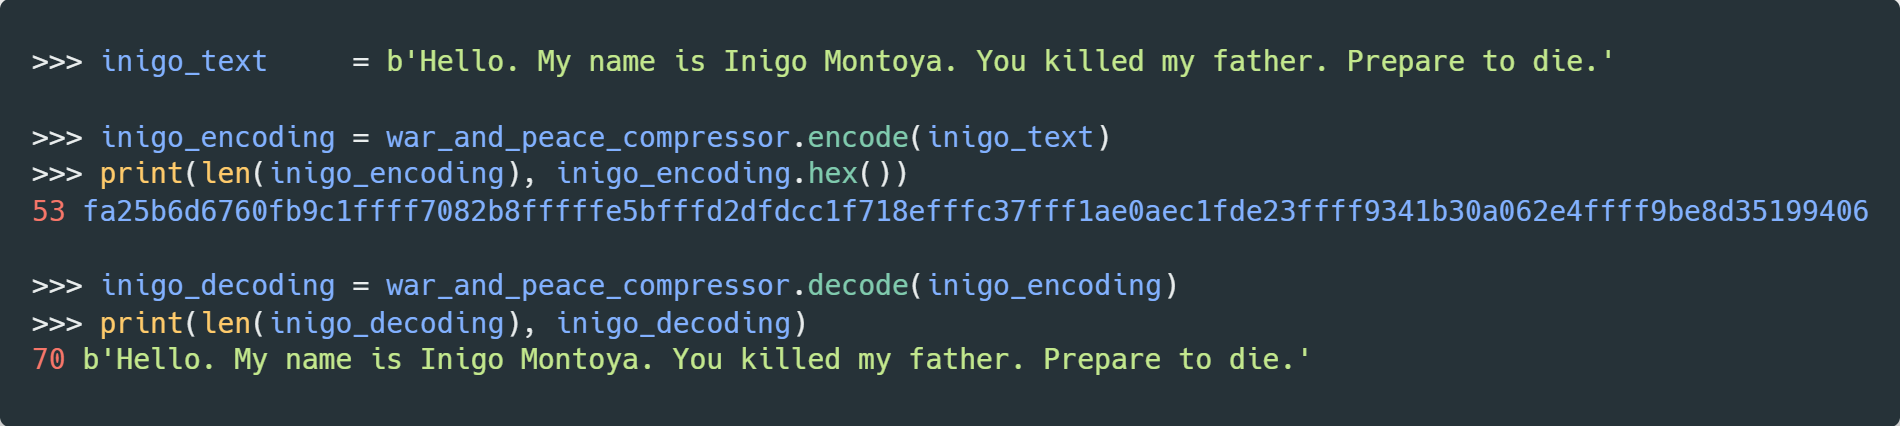
\includegraphics[width=\textwidth]{img/inigo_encoding_decoding.png}
\caption{Using WPC to encode and decode a few sentences.}
\label{fig:inigo_encoding_decoding}
\end{figure}

It is also possible to use the \texttt{decode} method on randomly generated bytes to obtain text that follows the regularities which the predictor has learned, as in Figure \ref{fig:predictor_decoding_randomness}.

\begin{figure}[h]
\centering
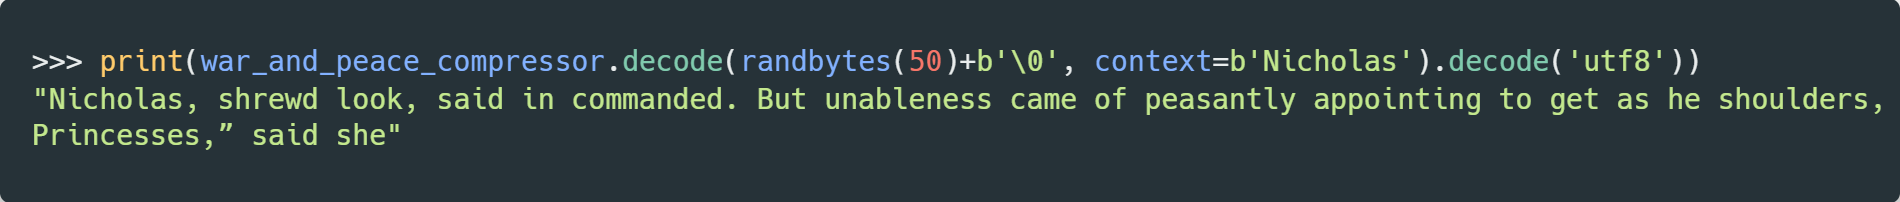
\includegraphics[width=\textwidth]{img/predictor_decoding_randomness.png}
\caption{Using the \texttt{decode} method on a randomly generated input}
\label{fig:predictor_decoding_randomness}
\end{figure}

The performance of a \texttt{Predictor} object depends on the text it has been trained on, and words and expressions which it is familiar with would therefore have shorter representations in its output encoding. For example, Figure \ref{fig:predictor_surprisal_by_char} shows the surprisal of \texttt{war\_and\_peace\_predictor} when trying to predict the characters in the first paragraph of The Adventures of Sherlock Holmes.

\begin{figure}[h!]
\centering
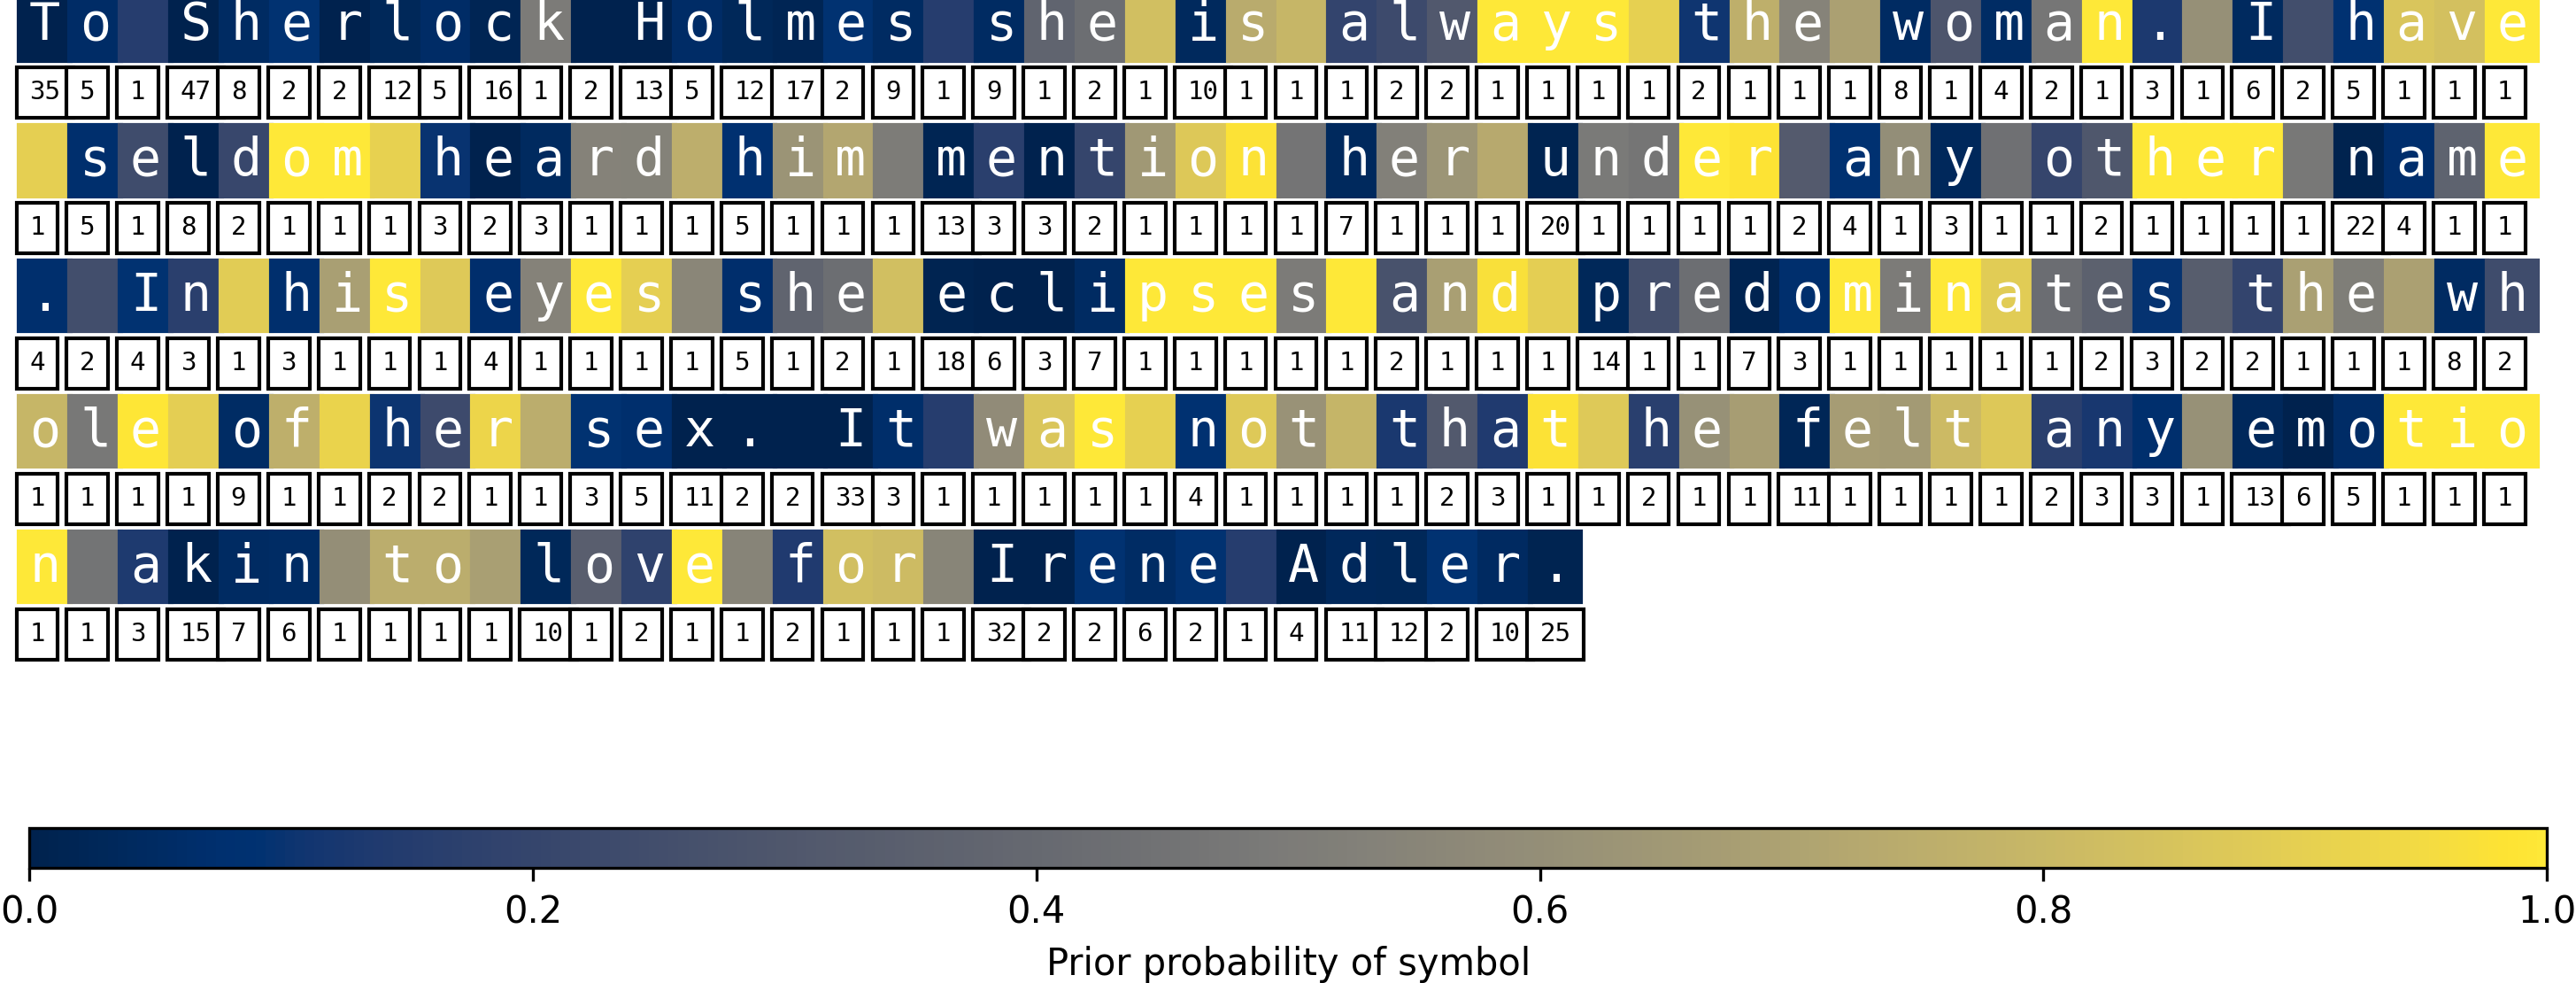
\includegraphics[width=\textwidth]{img/predictor_surprisal_by_char.png}
\caption{Surprisal of the \texttt{war\_and\_peace\_predictor} at each symbol in the opening passage of Sherlock Holmes. The prior probability given by the model to each symbol is indicated by its color, while how highly it ranked this symbol in terms of probability is indicated by a number below the symbol.}
\label{fig:predictor_surprisal_by_char}
\end{figure}

A few observations on Figure \ref{fig:predictor_surprisal_by_char},

\begin{itemize}
    \item For the first few symbols, the predictor performs badly as it has no context from which to infer the next symbol.
    \item The predictor performs especially badly for proper nouns. This is to be expected, as the words "Sherlock Holmes" and "Irene Adler" are not ones which it would have come across in War and Peace.
    \item The letter "k" at the end of "Sherlock" was expected with 0.5 probability by the model. On further investigation it seems this is because the 5-gram "erloc" appears in W\&P twice, in the words "interlocutor" and "interlocking", and half of these have a "k" following "erloc".
    \item The predictor often performs better on the ending of words than their beginning.
    \item For commonly found phrases such as "was not that he", the predictor's first guess for the following letter is very often correct.
\end{itemize}

Figure \ref{fig:predictor_surprisal_by_char} gives the probability rank of each symbol underneath it. For example, a rank of 2 indicates that the symbol would have been the predictor's second guess based on the previous 5-gram.

Figure \ref{fig:predictor_surprisal_histogram} and Table \ref{tab:predictor_surprisal} show the rank distribution when encoding the entire text of The Adventures of Sherlock Holmes.

\begin{figure}[h]
\centering
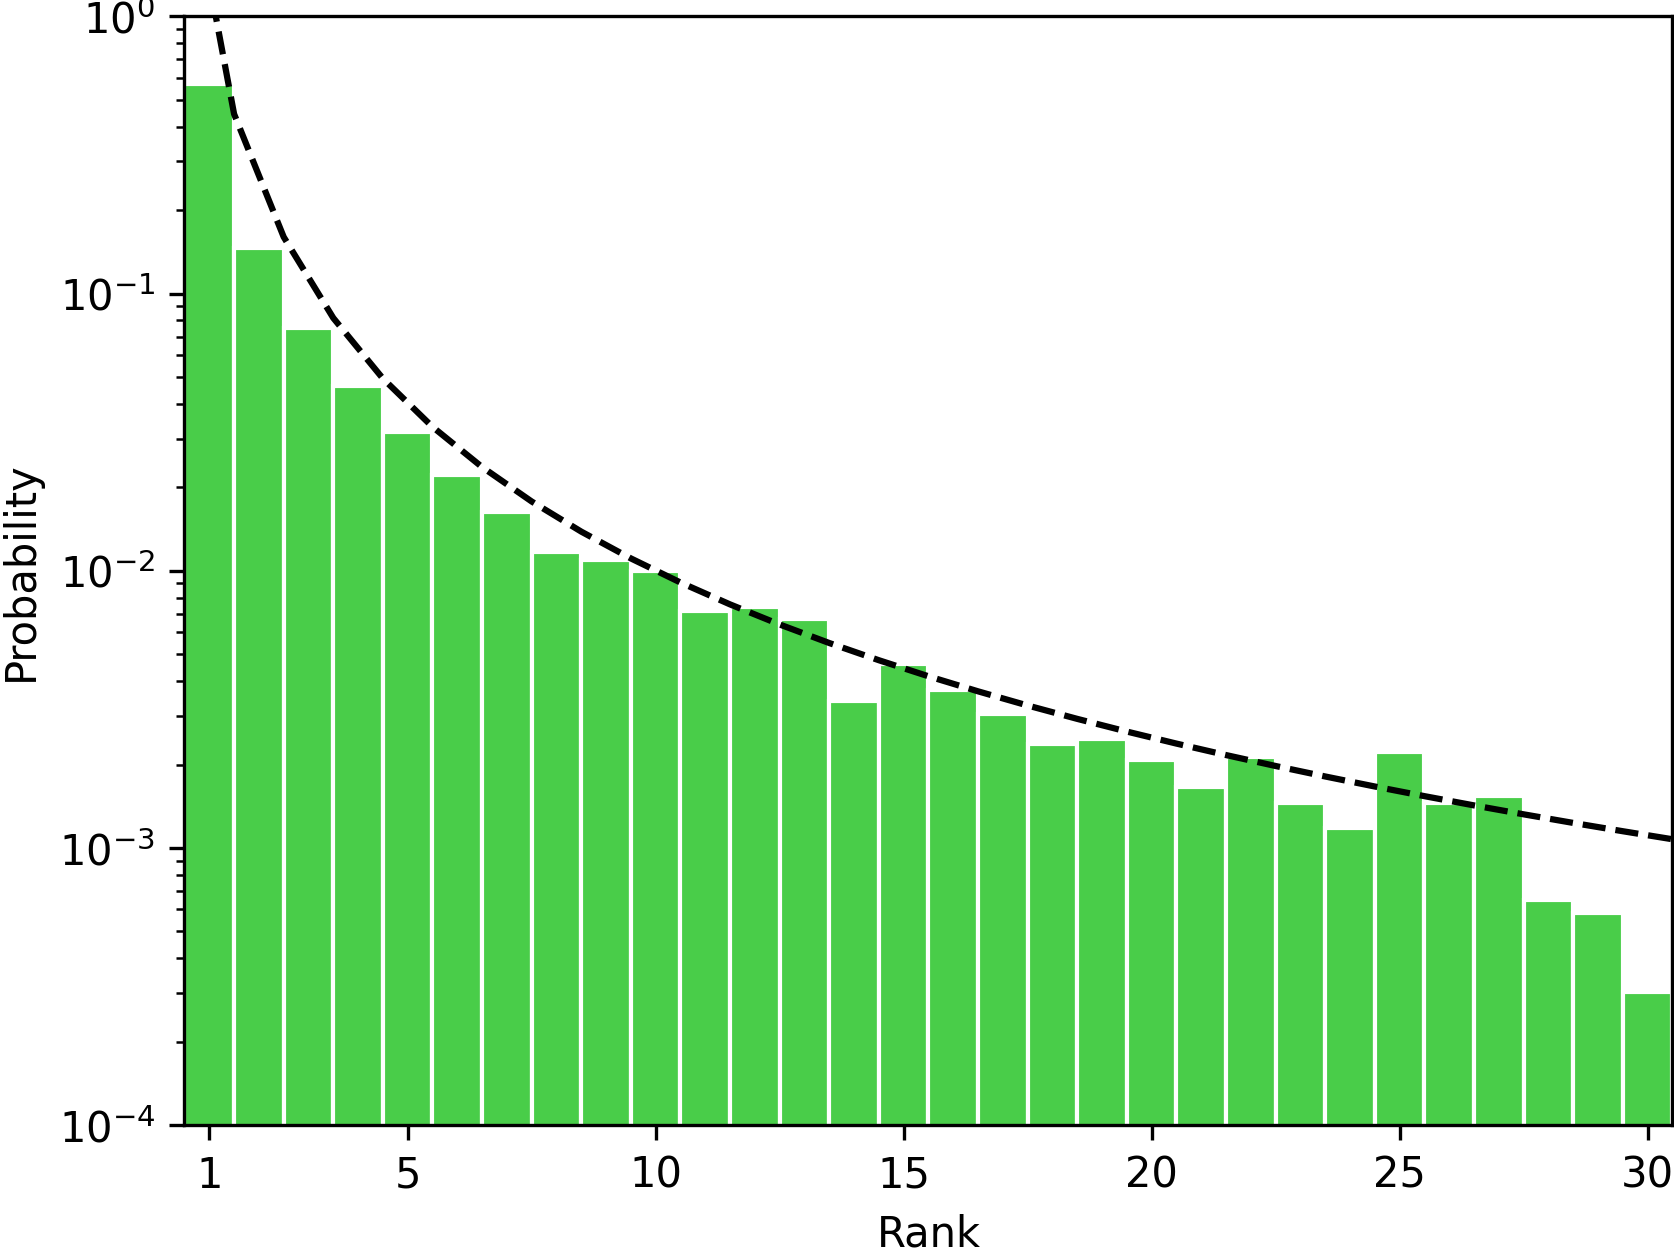
\includegraphics[width=\textwidth]{img/predictor_surprisal_histogram.png}
\caption{In this histogram, each bin represents a symbol rank from 1 to 30, and the height of the bin represents the frequency at which this rank occurs in the WPC's encoding of The Adventures of Sherlock Holmes. The dashed line shows the probability density function for the Pareto distribution with a scale of 1 and a shape of 1.}
\label{fig:predictor_surprisal_histogram}
\end{figure}

\begin{table}[ht]
\centering
\begin{tabular}{ |p{4cm}||p{1.5cm}|p{1.5cm}|p{1.5cm}|p{1.5cm}|p{1.5cm}|  }
 \hline
    Rank & 1 & 2 & 3 & 4 & 5\\
 \hline
    Probability & 0.568561 & 0.146148 & 0.075059 & 0.046406 & 0.031536\\
 \hline
    Human performance & 0.58 & 0.19 & 0.05 & 0.01 & 0.04\\
 \hline
    Zeta distribution ($6/{{\pi^2}{r^2}}$) & 0.607927 & 0.151982 & 0.067547 & 0.037995 & 0.024317\\
 \hline
\end{tabular}
\caption{In the first row, this table shows how often the WPC is correct in its first guess, second guess, etc. for the last letter in a 6-gram. The second row gives values given by \textcite{Shannon1951} obtained through experiments with English speakers similarly given 5 letters of context and asked to predict the full 6-gram. The third row gives the values of the zeta distribution with parameter 2 for comparison.}
\label{tab:predictor_surprisal}
\end{table}


The predictor trained on War and Peace accurately predicts a symbol based on the previous 5-gram on its first try 56.86\% of the time, and the frequency of the ranks follows a Pareto distribution with a scale parameter of 1 and a shape parameter of 1, i.e. the probability density function is $1/r^2$. The values for the discrete version of this distribution (the zeta distribution with parameter 2) is included in Table \ref{tab:predictor_surprisal} for comparison.

When initializing a \texttt{Compressor} object, one has a choice between using Huffman coding or arithmetic coding (by passing either the \texttt{Huffman} or the \texttt{Arithmetic} class as a parameter). These differ in how they assign binary codes to symbols, with Huffman coding being more economical - the average code length being usually minimal - and arithmetic coding being "fairer", in the sense that a symbol with $2^{-n}$ probability of occurring would have a code that is approximately $n$ bits long, that is, it preserves the probability distribution of the symbols.

For example, if symbol "a" occurs with probability 0.9 and symbol "b" appears with probability 0.1, Huffman coding would assign them the codes "0" and "1" respectively, while arithmetic coding would assign them "0" and "11101". Because of this difference, decoding a random sequence of bits using the Huffman code would result in an output which has an equal number of "a"s and "b"s, whereas decoding the same input using the arithmetic code would result in an output that is approximately 90\% "a"s and 10\% "b"s per the original distribution.

Table \ref{tab:6WPP_performance} shows the performance of WPC on some input texts using each code. For all examined texts (including Don Quixote, which is not in English), the compressed version is no larger than the original, and in fact this method typically performs better than gzip and zlib (see Table \ref{tab:compalg_benchmarks}). As expected, Huffman coding yields significantly better results than arithmetic coding. Note also that (apart from its own basis text), WPC performs best on the text of Crime and Punishment, which is the text that is closest to it historically and geographically, and which is therefore likely to contain many of the same regularities.

\begin{table}[h!]
\centering
\begin{tabular}{|l|c|c|}
 \hline
    Text & \makecell{Huffman\\compression ratio} & \makecell{Arithmetic\\compression ratio}\\
 \hline
    War and Peace                             &  4.258278  &  3.404772\\
    Crime and Punishment                      &  3.019220  &  2.068427\\
    Alice's Adventures in Wonderland          &  2.946588  &  2.028157\\
    Middlemarch                               &  2.895632  &  1.950565\\
    The Count of Monte Cristo                 &  2.894389  &  1.947010\\
    Don Quixote                               &  2.715589  &  1.833225\\
    The King James Version of the Bible       &  2.284923  &  1.543722\\
    The Complete Works of William Shakespeare &  1.984536  &  1.289506\\
 \hline
\end{tabular}
\caption{\label{tab:6WPP_performance}}
\end{table}

\subsection{Discussion}

For this section I constructed a versatile codebase inspired by Figure \ref{fig:twin_communication} (implemented in the \texttt{Predictor}, \texttt{Code}, and \texttt{Compressor} classes) and used it to verify some of the intuitions given in the \hyperref[chap:overview]{overview} as well as construct a simple compression method based on this framework that seems to outperform both gzip and zlib. I also note a pattern in Figure \ref{fig:predictor_surprisal_histogram} that requires further analysis.

As shown in Table \ref{tab:predictor_surprisal}, the performance of \texttt{NGramPredictor} is very close to that of humans when given the same amount of context, indicating that in principle, a code rate approaching that of humans when given 100+ characters of context (estimated around 1 bit / character) should be achievable. Of course, using an n-gram predictor for such a large context size is infeasible as the corresponding lookup table would need to contain something on the order of $26^{100}$ entries. Another algorithm would need to be used, and the next section examines the use of neural network-based machine learning models for this task.

Although NN-based predictors should have the advantage of detecting many subtle regularities in text, and of detecting relevant bits of context for themselves, using a hardcoded technique like n-gram prediction has some advantages: it is much faster to train, requires less data, and is interpretable.

Hardcoded techniques can be improved with a different (and not necessarily larger) choice of context. For example, as part of his experiments with English speakers, Shannon finds that knowledge of the n-gram that follows a character is approximately as useful as knowledge of the n-gram that precedes it when guessing what the character is, and it may be possible to create an algorithm that combines both forward- and backward-prediction, using the advantages of each.

Context also need not be constrained to adjacent characters, and I account for this in my \texttt{Predictor} superclass, giving it a method (\texttt{context()}) which allows it to update its internal state in an arbitrary way on reading a new byte. As simple examples, this can be used to store features such as whether the last character was punctuation, whether the last read word was capitalized, and perhaps the part of speech (noun, verb, etc.) of the last seen words using existing tools such as the \texttt{nltk} library's \texttt{pos\_tag()} method.

Another possible variation on this method is for the unitary symbols of context in use to be words instead of single characters, and Table \ref{tab:n_word_entropy} indicates that this should significantly improve compression.

Another point of interest in the data above is the distribution found in Table \ref{tab:predictor_surprisal} and Figure \ref{fig:predictor_surprisal_histogram}, which very closely approximates a zeta distribution with parameter 2 (only deviating at the right edge of the plot where data is sparse and therefore more prone to noise). This simply means that, in Figure \ref{fig:predictor_surprisal_by_char} for example, the number of characters marked with probability rank $r$ is inversely proportional to $r^2$. Why this should apply specifically in the case where n=6 is not clear, and it is possible that the parameter of the distribution is a function of $n$. Another datapoint that may help shed some light on deeper investigation of this distribution is that single words follow a well-known distribution given by Zipf's law, where the probability rank of a word $r$ is inversely prorportional to $r$ (note the difference in exponent).

Lastly, I use Figure \ref{fig:predictor_decoding_randomness} to propose a speculative explanation for the neurological condition of confabulation as seen in split-brain patients. These are patients in which the corpus callosum (a relatively thin channel connecting the two hemispheres of the brain) has been severed. \textcite{gazzaniga1967split} writes about a split-brain patient whose left (speaking) hemisphere is asked to give an explanation for an action made by his right hemisphere, and who proceeds to give an (unknowingly) confabulated but plausible explanation. I propose that since the two halves of the brain communicate over a thin channel, it is likely that encoding and decoding of information is taking place, and that therefore a severing of this channel would lead to noise being interepreted as plausible signal in the same way that the WPC decodes noise to text in the figure.

\section{Machine learning-based compression}
\label{sec:machine_learning}

As discussed in the previous sections, any mechanism which can detect regularities in a stream of data and predict future observations (symbols) from past ones (context) can also be used for compression by using it to estimate the probabilities of potential future observations and using these to assign shorter codes to the most likely of them.

While n-gram language models are very simple and easy to train, they are limited by their pre-specified (and often short) context, namely the previous [n-1] symbols in a text, with symbols being either characters or full words. For this reason, statistical models such as n-gram language models have generally been superseded by neural network-based models such as recurrent neural networks (RNNs), long short-term memory models (LSTMs), and most recently large language models (LLMs) such as BERT and GPT, which can retain information across larger contexts and better capture long-range dependencies in a text.

For RNNs, this is accomplished by having the network's previous outputs act as additional inputs when it observes a new symbol, giving it a simple form of memory. An improvement on this model is LSTMs, which are a subtype of RNNs that can learn to select relevant information to keep within its memory, and which generally outperform simple RNNs. Lastly, transformer-based LLMs use an attention mechanism to weight the relative importance of all words in the input data when making a prediction.

In this section I perform simple experiments with one simple RNN and one LSTM, once again subclassing the \texttt{Predictor} class and plugging it (as well as an entropy coding) into a \texttt{Compressor}. The code for this section can be found at \texttt{\href{https://github.com/Guy29/FYP/blob/main/Code/machine_learning}{Code/machine\_learning}}.

As before, it is possible to feed the \texttt{decode} method noise to see what regularities the model has learned about.

\begin{figure}[h]
\centering
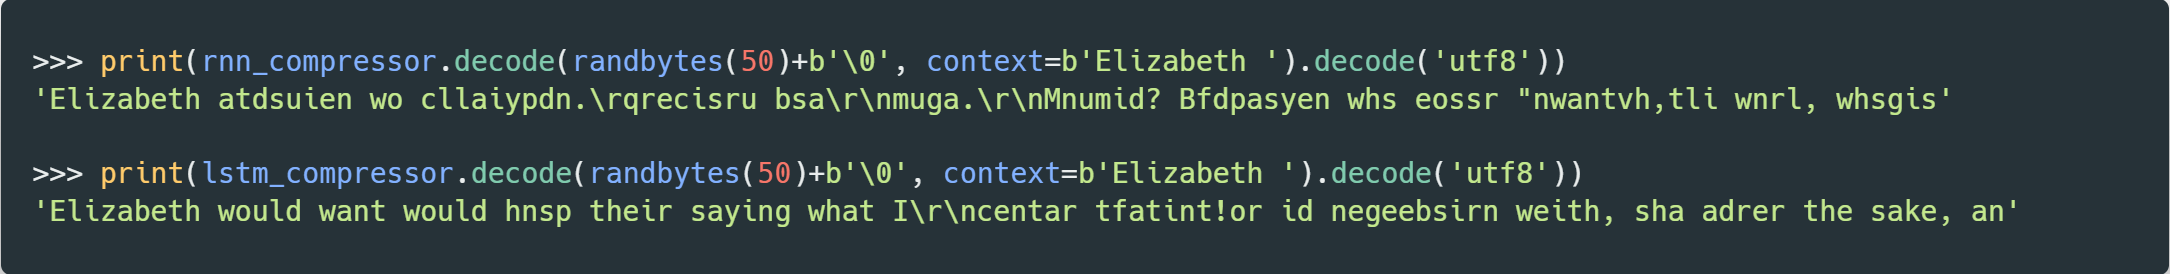
\includegraphics[width=\textwidth]{img/ML_decoding_randomness.png}
\caption{Using the \texttt{decode} method on a randomly generated input}
\label{fig:ML_decoding_randomness}
\end{figure}

With both models the text is much less coherent than with the n-gram model, although the models have still learned which byte values are characters, how often spaces are used, some common collocations, and in the case of the LSTM model some common words. It is likely that with more training or a wider context window the models would be better able to capture the regularities in English, but due to constraints on time and computational power it was not possible to test this in more depth.

As part of the process of training, my code serializes and saves the models periodically. One of the significant advantages of machine learning models over n-gram based models is that the trained version is much smaller (approximately 4 mb in the case of the LSTM and 1.5 mb in the case of the RNN).

My implementation of these models was unfortunately too slow to be practicable on large texts, although I suspect efficient implementations are possible. For an estimate of compression ratios, I use an excerpt from Sherlock Holmes, which neither model was trained on. This test indicates compression ratios of 1.253 and 2.008 for the RNN- and the LSTM-based compressors respectively.


\subsection{Discussion}

\todo[inline, color=yellow]{Mention autoencoders and latent spaces}

\todo[inline, color=yellow]{Write about potential use of LLMs, at least in future work subsection}

\section{Co-compression}
\label{sec:co_comp}

In sections \ref{sec:n_gram} and \ref{sec:machine_learning}, we explored leveraging an understanding of a text's regularities for compression. This section explores the opposite idea, namely using an existing compression algorithm as a black box to understand regularities in text.

One point of commonality between compression and comprehension is the need for parsimony. This is expressed by Occam's razor, which states that "entities must not be multiplied beyond necessity" and commonly understood to mean that "the simplest explanation is usually the best one".

Compression algorithms, for example the family of Lempel-Ziv algorithms, in fact operate by eliminating the multiplication of entities through the creation of a \emph{codebook}, a mapping between often-repeated bits of data and what is essentially an abbreviation for each. If the relationship between compression and comprehension holds, we should expect to be able to use an existing compression algorithm like LZMA to get a rudimentary understanding of text.

\textcite{Jiang2023} showed that it's possible to use gzip for text classification, based on

\begin{displayquote}
"the intuitions that
\begin{enumerate}
\item compressors are good at capturing regularity; 
\item objects from the same category share more regularity than those from different categories"
\end{enumerate}
\end{displayquote}

To illustrate this using the same dataset of 97 Gutenberg texts, I use the following scoring methods to estimate the similarity of a pair of texts:

\[add(y|x) = \frac{C(xy) - C(x)}{C(y)}\]

where \(C(t)\) is the compressed length of \(t\) expressed in bytes, and \(xy\) is the concatenation of the texts \(x\) and \(y\). The function \(add(y|x)\) is then a measure of the additional information given by \(y\) when \(x\) is taken as a known basis.

To give an intuition for why the measure is defined in this way, it's helpful to use an example. Suppose that $x$ is the text of the complete works of Shakespeare and that $y$ is the text of Romeo and Juliet. Since $x$ contains $y$ as a substring, we should expect that a good compression algorithm would compress the concatenation $xy$ in little more space than is required for just $x$, as the entire text of $y$ can be signified with a single symbol in the codebook, compressed once, and referred to twice.

Because of this, we should expect the value of $add(y|x)$ in this case to be close to 0, corresponding to the fact that $y$ does not really add information to $x$. Conversely, since the complete works of Shakespeare contain a lot of information not contained in just Romeo and Juliet, we should expect $add(x|y)$ to be close to 1, indicating that our compression algorithm's knowledge of the text of Romeo and Juliet only makes a small dent in the number of additional bits it needs to represent the works of Shakespeare.

The measure used above contrasts with Normalized Compression Distance (NCD) as used by \textcite{li2004similarity} , in that it is directional, i.e. that \(add(x|y)\) is not necessarily equal to \(add(y|x)\).

We may also define a more intuitive similarity score as follows

\[similarity(y|x) = 1 - add(y|x) = \frac{C(x) + C(y) - C(xy)}{C(y)}\]

This score giving a measure of the similarity of \(y\) to \(x\). In this case, $similarity(a|b)=1$ would indicate that $a$ is fully described by $b$ (as it contains no additional information), and $similarity(a|b)=0$ indicates that $a$ is unlike anything seen in $b$. Again, note that \(similarity(y|x)\) is not necessarily equal to \(similarity(x|y)\).

\begin{figure}[t]
\centering
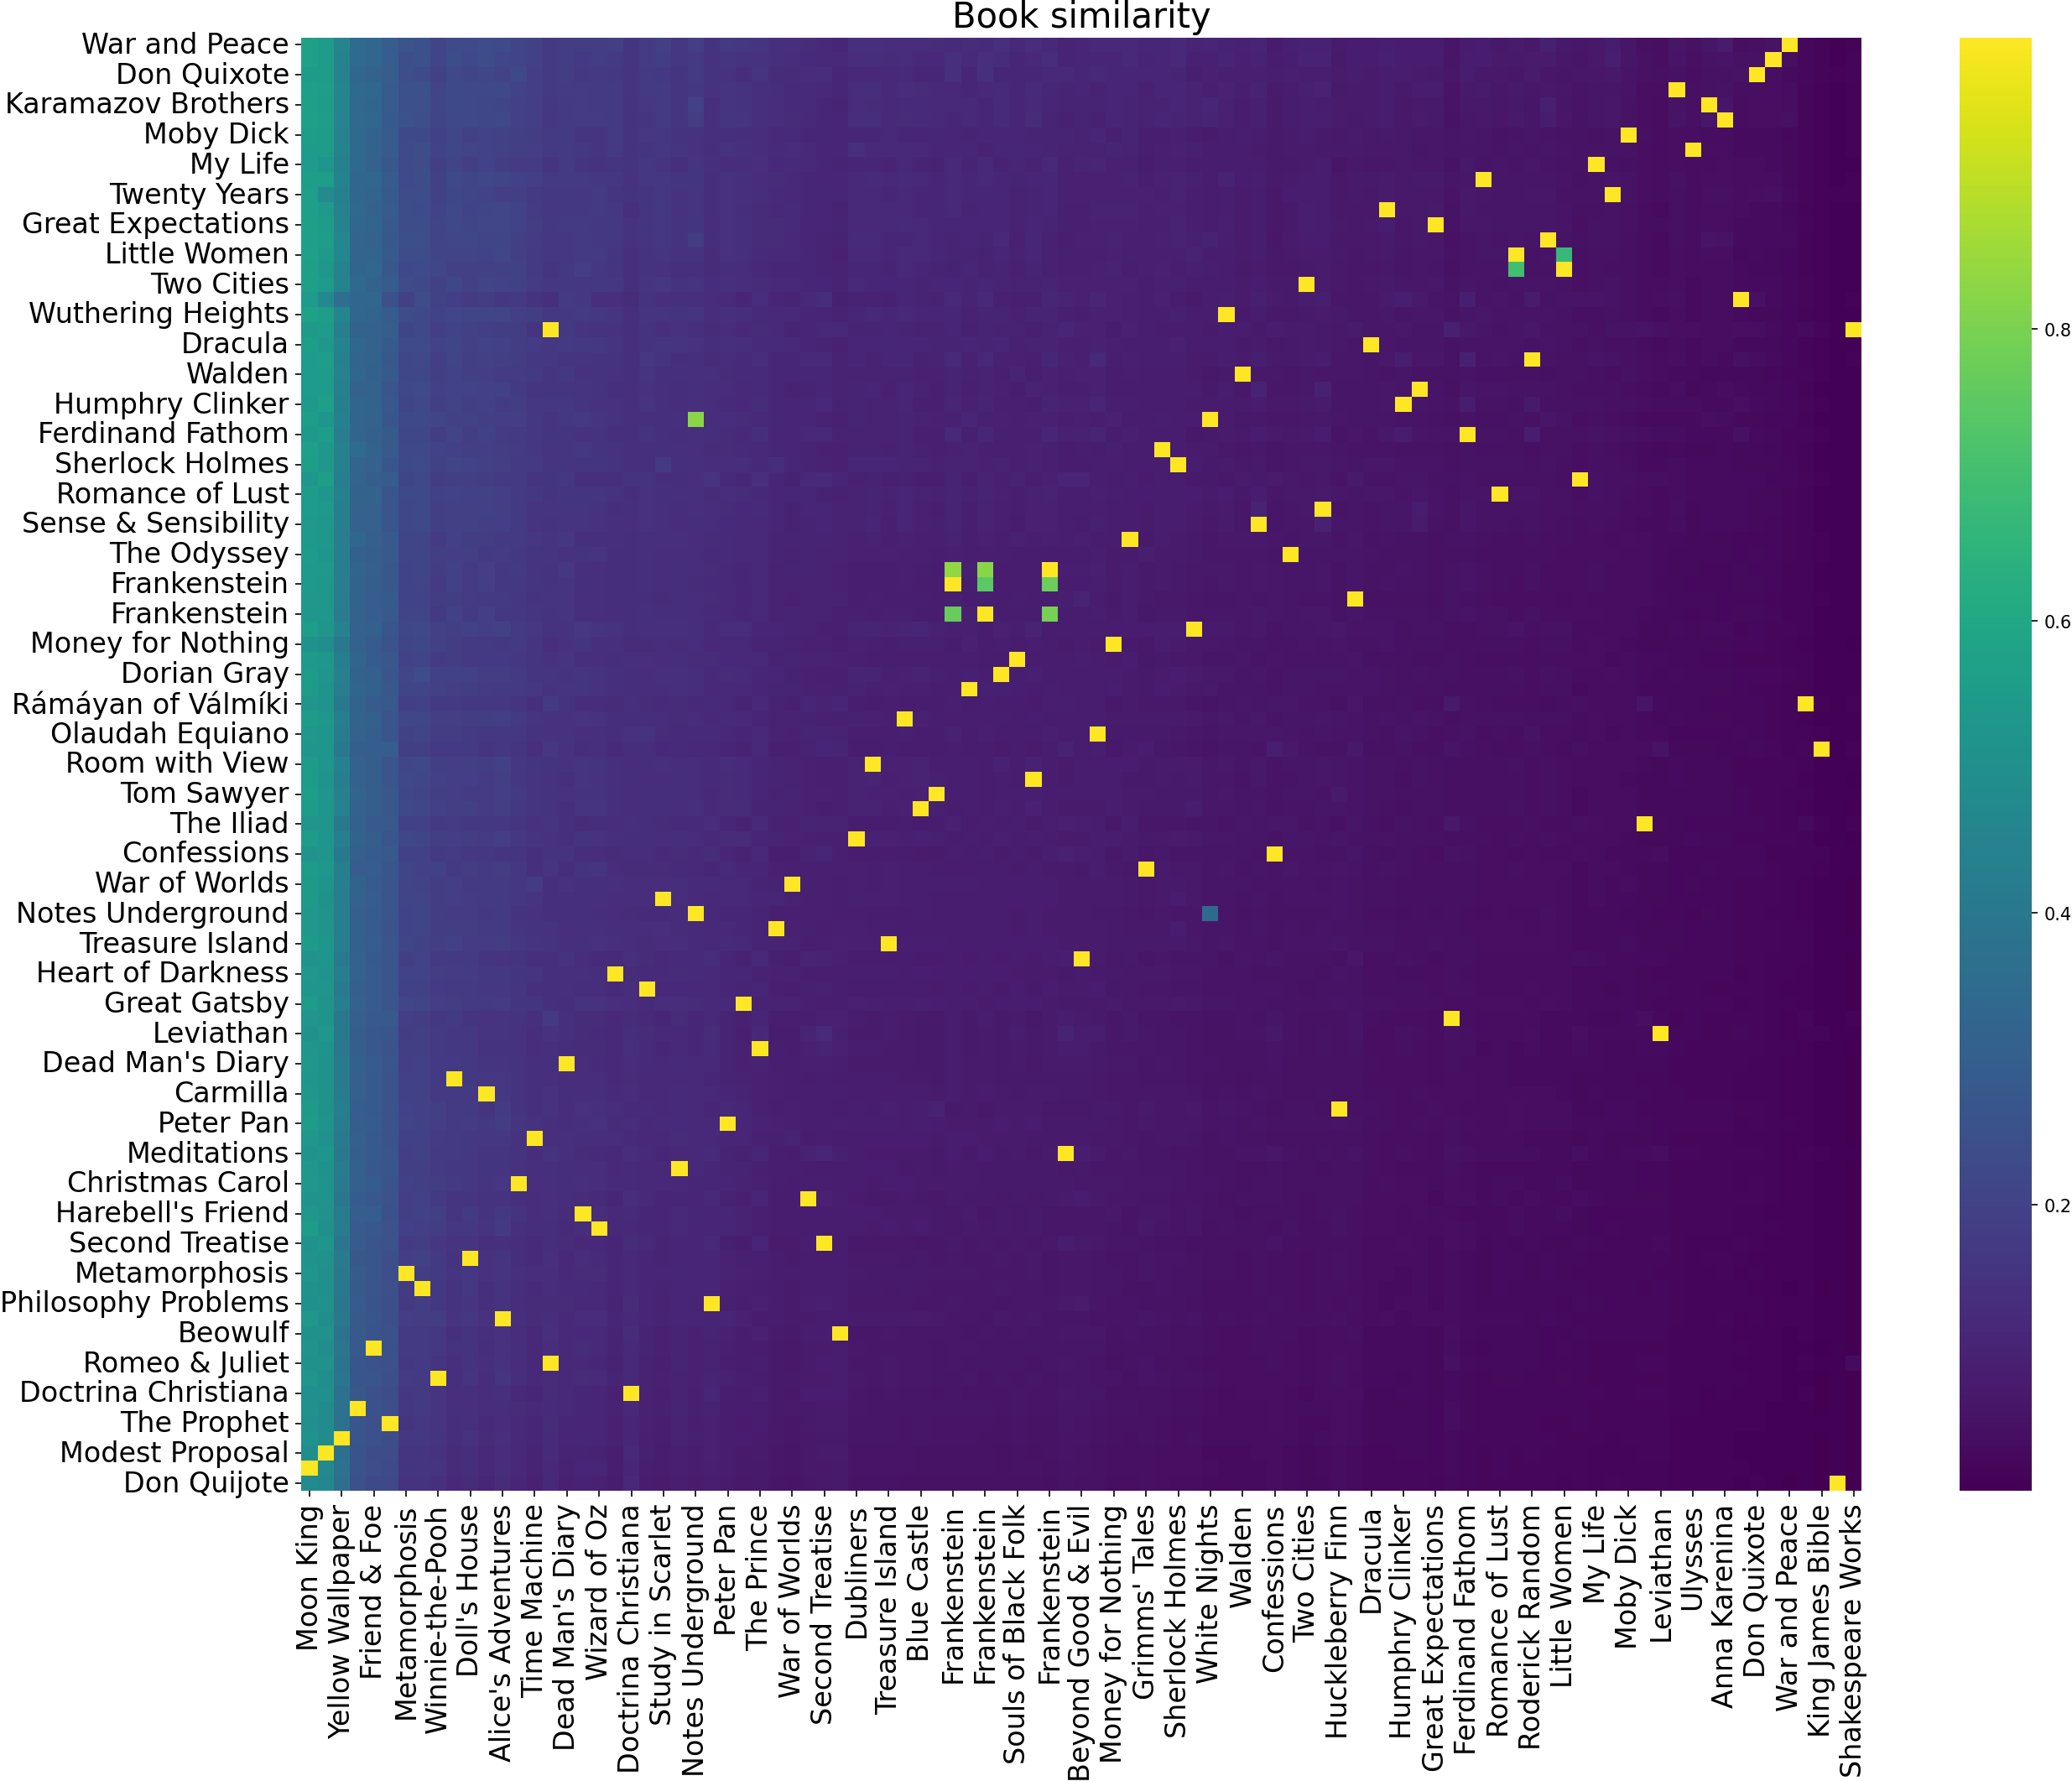
\includegraphics[width=\textwidth]{img/fig_co-compression_median.png}
\caption{Similarity scores for pairs of texts. The texts on the vertical axis are ordered most-predictive-first, and those on the horizontal axis are ordered most-predictable-first.}
\label{fig:heatmap_ppsort}
\end{figure}

\begin{figure}[t]
\centering
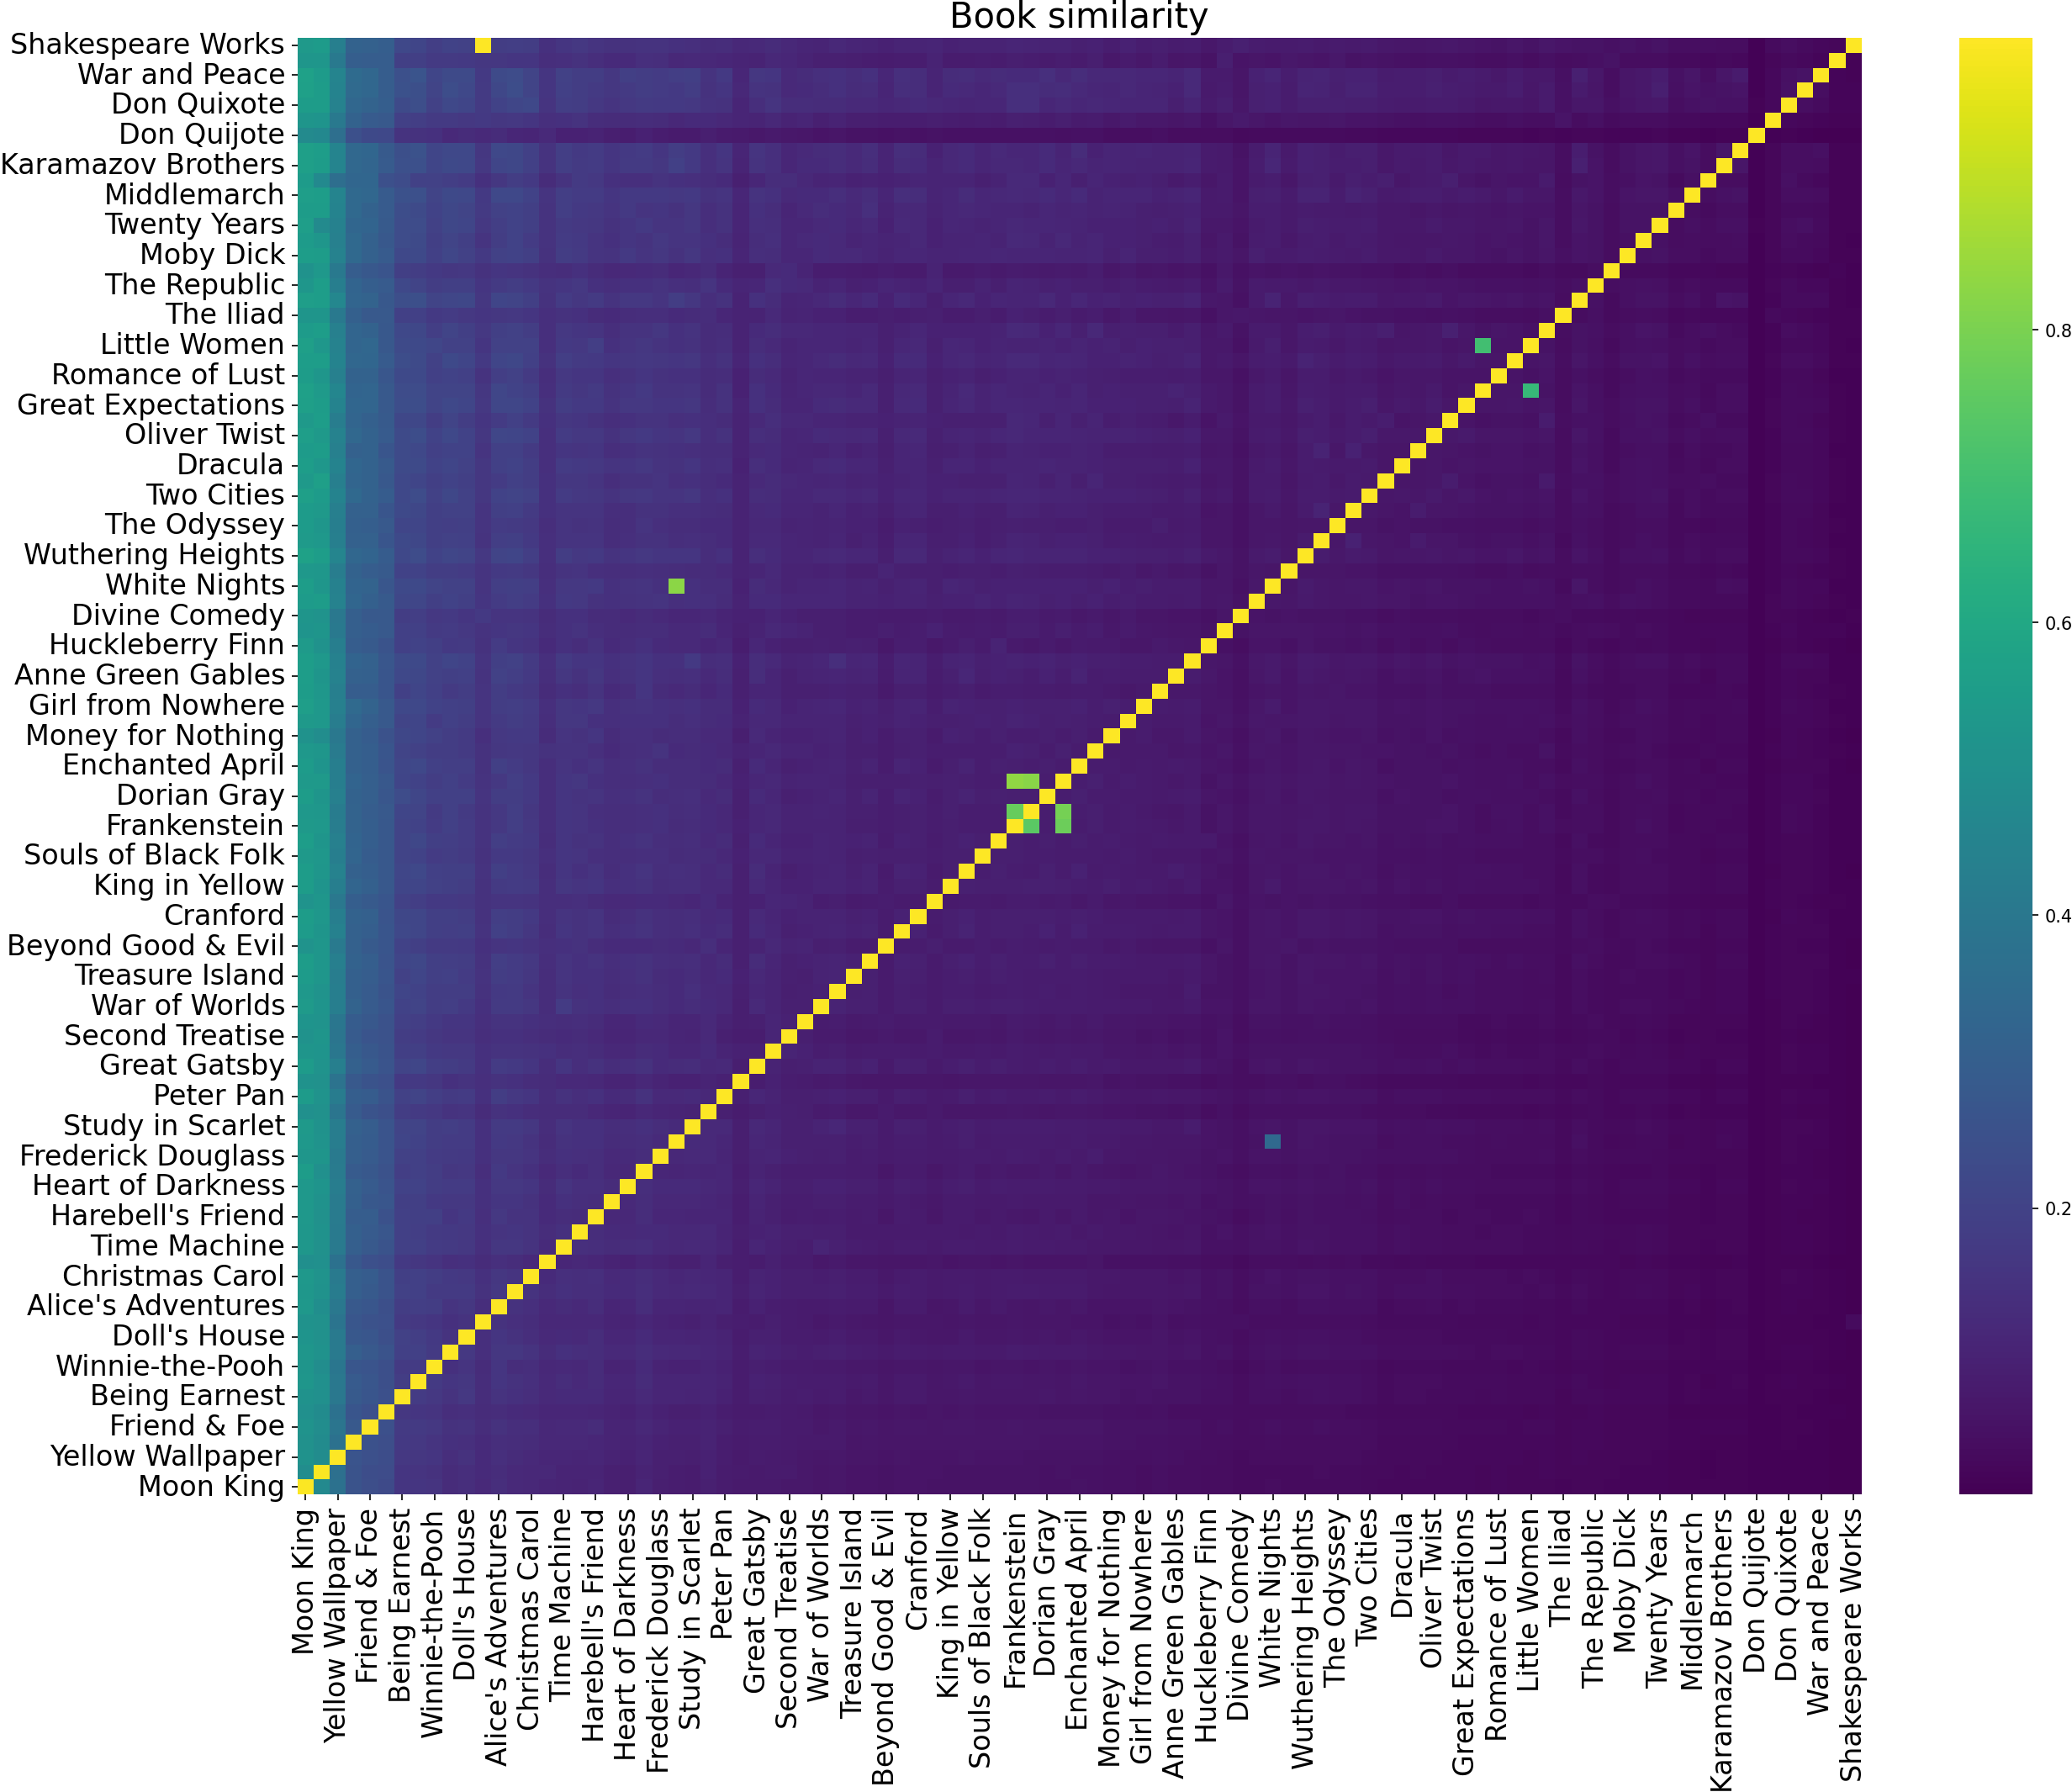
\includegraphics[width=\textwidth]{img/fig_co-compression_file_size.png}
\caption{Similarity scores for pairs of texts. The texts on both axes are sorted by file size.}
\label{fig:heatmap_fsort}
\end{figure}

This similarity score is plotted for pairs of texts in Figures \ref{fig:heatmap_ppsort} and \ref{fig:heatmap_fsort}, each plot giving \(x\) on the horizontal axis and \(y\) on the vertical axis, the color of the cell representing \(similarity(x|y)\). In Figure \ref{fig:heatmap_ppsort}, the texts on the vertical axis are sorted by how predictive they are on average, and the texts on the horizontal axis are sorted by how predictable they are. In Figure \ref{fig:heatmap_fsort}, the same texts are instead sorted by file size on both axes.

The figures are produced in the  \texttt{\href{https://github.com/Guy29/FYP/blob/main/Code/co_compression/stats.py}{co\_compression/stats.py}} script in the repository for this project. Creating the figures involved experimenting with each of 4 compression algorithm libraries (\texttt{zlib}, \texttt{lzma}, \texttt{gzip}, and \texttt{bz2}) to find the most suitable for co-compression. Since one of the functions that \texttt{stats.py} performs is to co-compress all possible pairings of texts from a set of 97, the results are serialized and saved regularly to avoid need for recalculation. The script uses the \texttt{seaborn} and \texttt{matplotlib} python libraries for generating the figures, and \texttt{pandas} is used to process and tabulate the data.

The following observations can be made based on Figures \ref{fig:heatmap_ppsort} and \ref{fig:heatmap_fsort}:
\begin{itemize}
  \item In general, larger texts are more predictive.
  \item In general, smaller texts are more predictable.
  \item There are a few very bright dots which do not lie along the diagonal in \ref{fig:heatmap_fsort}. These appear because the dataset includes three versions of Frankenstein which have a high similarity score with each other, as well as the texts for Romeo and Juliet, and the Complete Works of Shakespeare. For this last pair, the latter strongly predicts the former but the former only weakly predicts the latter. The same applies to White Nights and Notes from the Underground, where the former contains the latter.
  \item There is a strong horizontal dark line in both graphs, which represents a text that is unpredictable regardless of what other text it is paired with. On inspection, this turns out to be Don Quijote, which is in fact unlike the other texts because it is in Spanish, whereas most other texts are in English.
  \item As can be seen in \ref{fig:heatmap_ppsort}, when texts are sorted most-predictive-first on the $y$-axis and most-predictable-first on the $x$-axis, texts generally lie along the diagonal. This indicates that, within a set of texts, there is a trade-off between how predictive a text is and how predictable it is. At least part of this effect has to do with file size, as larger texts tend to contain a larger set of the possible words and expressions of a language.
  \item There is a visible pattern of strong vertical and horizontal lines in \ref{fig:heatmap_fsort} (i.e. there is a low level of noise), indicating that texts tend to be "generally predictive" or "generally predictable" within a given collection.
\end{itemize}

\subsection{Practical application}
\label{subsec:co_comp_practical}

As can be seen in the previous figures, it is always the case for any two pairs of texts $x$ and $y$ that "the whole is less than the sum of its parts", i.e. that $C(xy) \leq C(x) + C(y)$ (note the similarity to the triangle inequality). This opens up the question of whether it is possible to obtain a better compression of $y$ by encoding only that information which it adds to $x$. If this is possible, we should expect that this information should be of the size $C(xy) - C(x)$ which, by the previous equation, is $\leq C(y)$.

Intuitively, this means that if two parties - Carol and Dave - each have a copy of the works of Shakespeare, and Carol wants to send over Romeo and Juliet, she can simply encode it by giving the range of pages on which it appears in their shared reference text, a much shorter representation than sending the actual text of Romeo and Juliet.

Is this possible to implement in practice? The fact that Lempel-Ziv algorithms work by going through the data in one pass and creating a codebook as they go indicates that $D(xy)$ should contain $D(x)$ as a prefix, where $D(t)$ stands for the compression of $t$. This is, in fact, more or less the case with LZMA, and I was able to create a simple tool that implements this idea, available at \texttt{\href{https://github.com/Guy29/FYP/blob/main/Code/libraries/co_compressor.py}{libraries/co\_compressor.py}} .

The \texttt{CoCompressor} class I implement is instantiated with two arguments: a reference text $r$ and a compression algorithm. Its \texttt{compress} method takes a text $t$ to compress and outputs $D(rt)$ with the prefix $D(r)$ removed, and its \texttt{decompress} method takes a text compressed in this way, prefixes it with $D(r)$ and decompresses it, reversing the process.

Co-compressors instantiated in this way differ in their power depending on the choice of reference text. See Figure \ref{fig:cocomp_comparison} below for a comparison of the performance of co-compressors trained on different reference texts.

\begin{figure}[h]
\centering
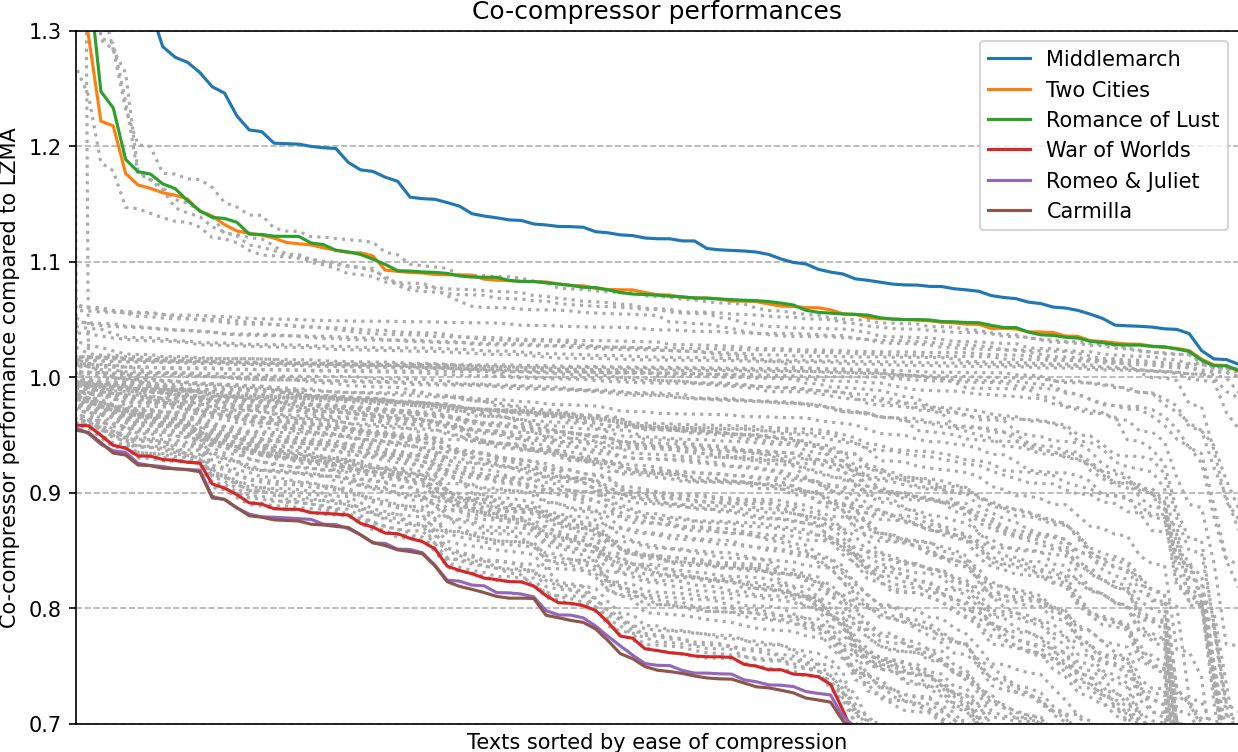
\includegraphics[width=\textwidth]{img/fig_cocomp_performance.png}
\caption{The performance of instances of the \texttt{CoCompressor} class trained on 97 different texts. Each line represents a \texttt{CoCompressor}. The value on the vertical axis is the Relative Compression Ratio (RCR), calculated as the size of the encoding produced by naive LZMA divided by that produced by the \texttt{CoCompressor}, while the horizontal axis goes through possible inputs for comrpession.}
\label{fig:cocomp_comparison}
\end{figure}

There are a few remarkable things about this figure:

\begin{itemize}
    \item Each co-compressor shows a tan- or sigmoid-like curve, performing exceptionally well on texts which are very similar to it (left side of the plot) and steeply dropping down in performance for sufficiently different texts.
    \item There is very little criss-crossing between the lines in this plot. That is, for any pair of co-compressors, one will usually outperform the other \emph{on every input} in the dataset. Why there should be a strict hierarchy of this sort is not clear, as one might expect that a specific co-compressor would be specialized for texts which are similar to it but not for others.
    \item The best performing co-compressor in this dataset is the one trained on Middlemarch (performing 12\% better than naive LZMA in the median case), followed by A Tale of Two Cities (7.3\%) and The Romance of Lust (7.2\%).
\end{itemize}

It is tempting to explain away the unusual performance of the Middlemarch co-compressor (henceforth $CC_{MM}$) as an artifact of the chosen dataset, that it might be situated (historically or otherwise) "in the middle" of the dataset, sharing some features with both preceding and following literary works.

One strong piece of evidence against this is that, as noted above, the performance of co-compressors is strictly hierarchical, and this effect extends all the way to the left of the plot where the co-compressor is fed the text it performs best on (that is, its own text) as its input. Examining this, we notice that

$$RCR_{MM}(MM) > RCR_t(t) \qquad \forall t \in G$$

where $RCR_a(b)$ is a measure of the performance of the co-compressor trained on text $a$ when fed input $b$ (as defined in Figure \ref{fig:cocomp_comparison}), and $G$ is the Project Gutenberg dataset. That is, $CC_{MM}$ is not only the most performant co-compressor on all the texts in the dataset, it is also the co-compressor that performs best on its own reference text.

This observation gives a simple way to find other good reference texts for co-compressors: one simply calculates $RCR_t(t)$ for each candidate and finds values of $t$ that yield the highest performance.

I implement this method on a much larger dataset of 92600 texts downloaded from Project Gutenberg, this time only using \texttt{CoCompressor} objects trained on a text to compress the same text, and measure the relative compression ratio (RCR) for each text, where

$$RCR_a(b) = \frac{length(LZMA(b))}{length(CC_a(b))}$$

that is, the performance of the co-compressor relative to naive LZMA.

\begin{figure}[h]
\centering
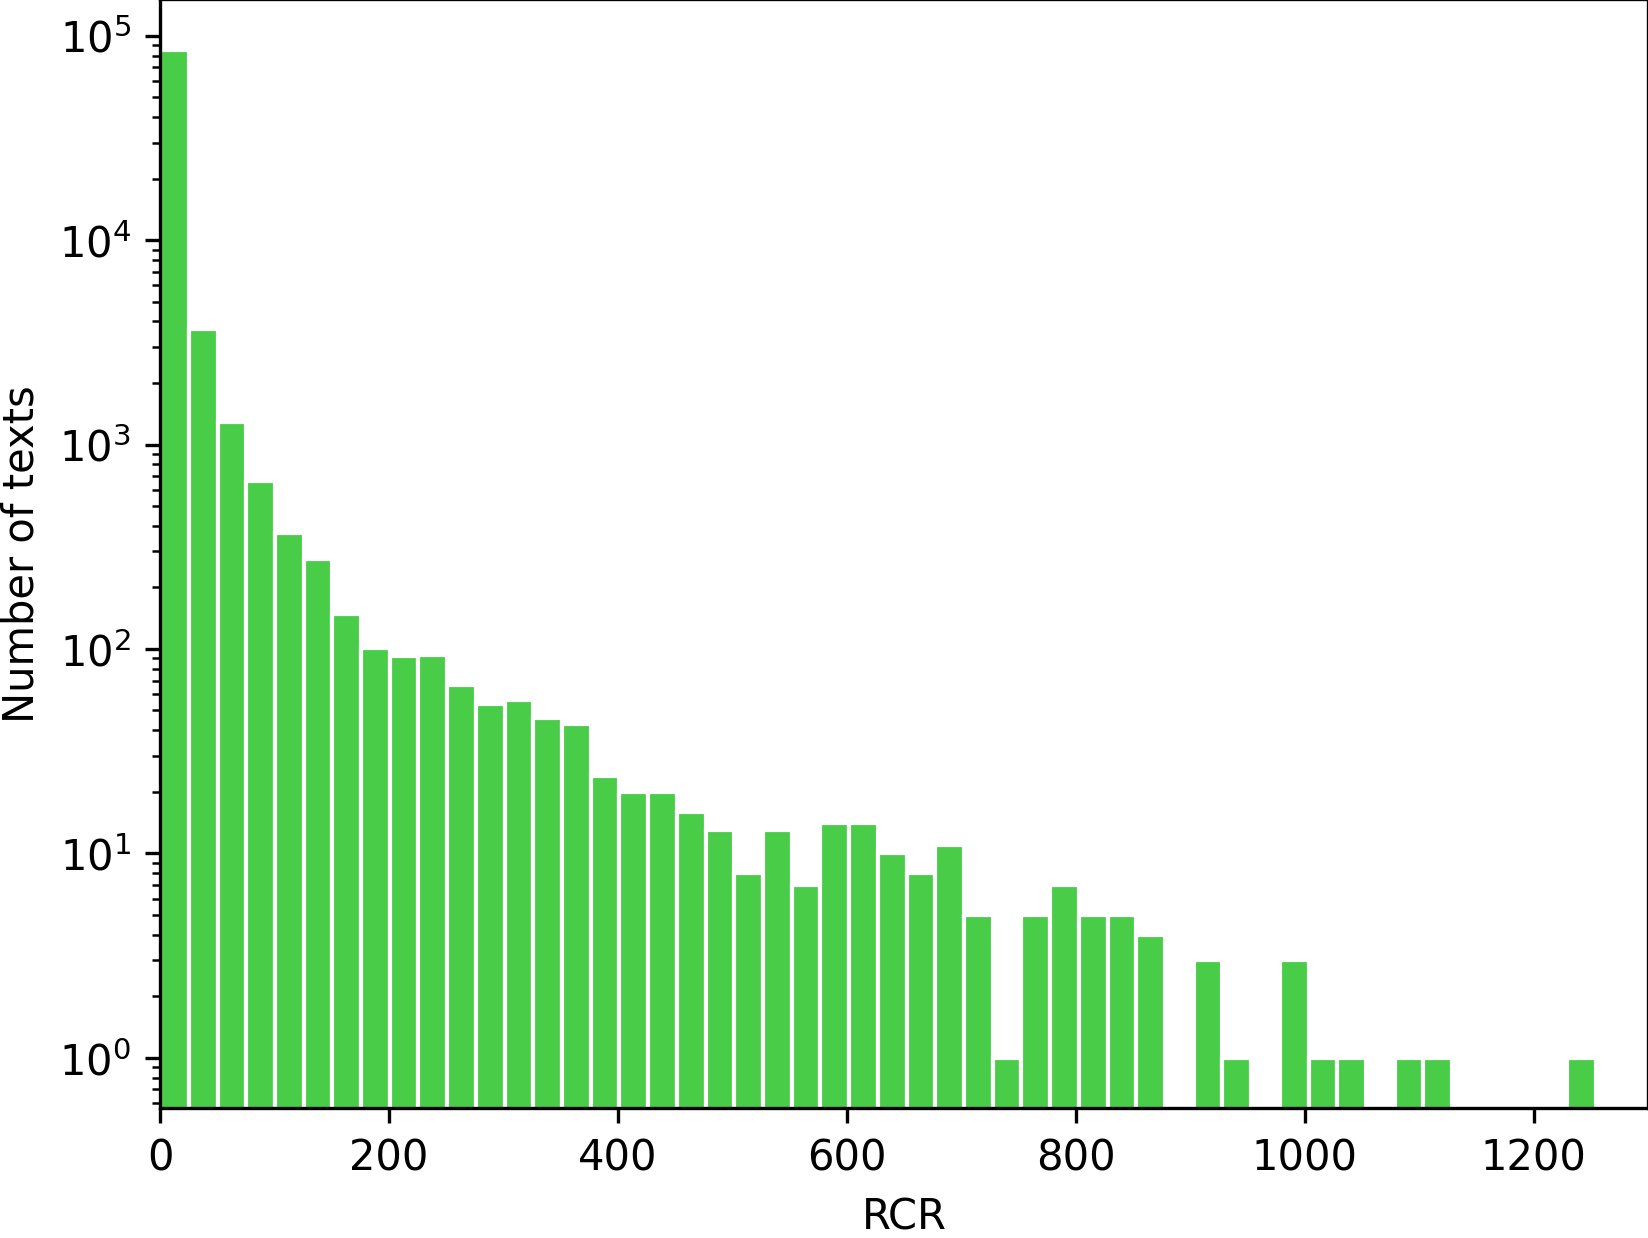
\includegraphics[width=\textwidth]{img/fig_self-compression_histogram.png}
\caption{A histogram representing the self-compression score (RCR) of 96200 Project Gutenberg texts.}
\label{fig:self_compression_histogram}
\end{figure}

Figure \ref{fig:self_compression_histogram} shows how the 92600 texts in this dataset cluster in terms of their RCR. Note that the vertical axis is logarithmic. If the hypothesis that texts with a high RCR are good co-compressors, we should expect some of them to outperform Middlemarch if Figure \ref{fig:cocomp_comparison} is re-plotted to include these texts.

This is, almost, what we find in Figure \ref{fig:cocomp_comparison_best}. The 30 texts with the highest RCR were selected for inclusion in this plot. As can be seen here, all of these outperform naive LZMA to some degree, with Middlemarch still performing best in the median case.

\begin{figure}[h]
\centering
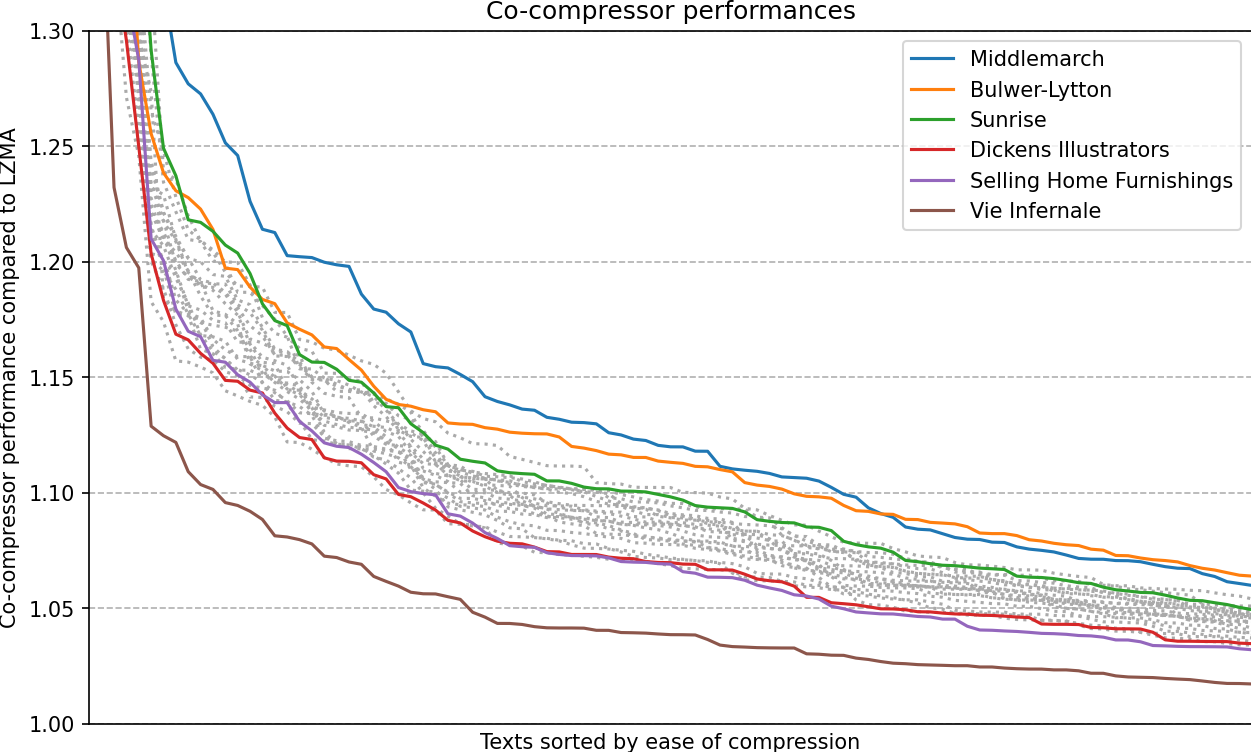
\includegraphics[width=\textwidth]{img/fig_cocomp_performance_best.png}
\caption{The performance of instances of the \texttt{CoCompressor} class trained on 30 texts selected for their high RCR out of a set of 96200 candidate texts. Each line represents a \texttt{CoCompressor}. The value on the vertical axis is the ratio of the size of the encoding produced by naive LZMA to that produced by the \texttt{CoCompressor}, while the horizontal axis goes through possible inputs for comrpession.}
\label{fig:cocomp_comparison_best}
\end{figure}



\subsection{Discussion}

In this section I examined specializing an existing compression algorithm on a given basis text to obtain an improved method of compression, as well as what choices of basis text perform best. The method is fully implemented and usable, and there is a selection of texts which always outperform naive LZMA, with Middlemarch being the best of these, outperforming LZMA by 12\% in the median case.

It is still not clear why George Eliot's Middlemarch, Edward Bulwer-Lytton's "My Novel", or William Black's Sunrise perform so well as a basis text, and one hypothesis (that it has most in common with the other texts in the initial 97-large dataset) is considered and disproved by showing that Middlemarch has a high RCR, which is a metric that considers each text on its own without reference to any other texts.

In fact, Émile Gaboriau's La Vie Infernale barely makes the cut for the top 30 texts in terms of RCR and still improves on naive LZMA by 4\%, as can be seen in Figure \ref{fig:cocomp_comparison_best}, even though it is written in French. It is, however, the worst performing text in this group by a significant margin.

A few avenues of investigation into this phenomenon come to mind, all of the form of performing some transformation on a high-performing basis text and measuring its performance after the transformation. For example, one may perform a caesar shift operation on the text of Middlemarch, or use a translation of it in a different language, or either truncate it or add some padding at the end to change the file size.

It may also be useful to experiment with automatic basis text generation, perhaps starting with random strings and examining the distribution of their RCRs, or by iteratively probing the RCR to check which characters it is best to extend the basis text with.

% Disable todo notes
%\let\oldtodo\todo
%\renewcommand{\todo}[2][]{}

\todo[inline, color=yellow]{Idea: see if there's a chain of bootstrapping. Middlemarch compresses everything well, but is there something that compresses Middlemarch well? If so, use that as an earlier step in the bootstrapping}
\todo[inline, color=yellow]{Idea: how well does the first half of Middlemarch compress the second half? If the resulting compression is short enough, this facilitates bootstrapping even more: use part 1 to compress part 2, use the total to compress another text. You could also do it in more splits.}
\todo[inline, color=yellow]{Idea: co-compressors take compressors as one of their initializers, but they are themselves compressors. Is there any use in stacking them?}
\todo[inline, color=yellow]{Idea: try to add some noise to a compressed version of something and see if it decompresses into anything}
\todo[inline, color=yellow]{Idea: if the \texttt{CoCompressor} class takes a compression algorithm and improves it, can this method be used recursively on itself (starting with some very naive compression) to get something that performs significantly better?}
\todo[inline, color=yellow]{Idea for practical compression: start compressed file by indicating what you want to use as a basis text, then give compressed version. Potentially, stack these: if you need basis A to get B and basis B to get C, have the file format allow passing both B and C using basis A.}

% Re-enable todo notes
%\let\todo\oldtodo

\section{Natural language compilation}

\subsection{Montague grammar}
In 1970, logician Richard Montague posited that there is “no important theoretical difference between natural languages and the artificial languages of logicians” and that it is “possible to comprehend the syntax and semantics of both kinds of language within a single natural and mathematically precise theory.” \autocite{Montague1970_universal_grammar} and \autocite{Montague1970_english_formal}

Montague gives a grammar which can be used to parse English, and a specification for a parser based on this grammar is given by Friedman \& Warren \autocite{Friedman1978}.

\todo[inline, color=yellow]{Scrap this section or move to chapter \ref{chap:discussion}}
\chapter{Discussion and future work}
\label{chap:discussion}

As each of sections \ref{sec:n_gram}, \ref{sec:machine_learning}, and \ref{sec:co_comp} includes its own specialized discussion, this chapter addresses only the approaches not explored before, as well as the bigger picture.

\section{Other avenues of investigation}

Firstly, one approach was considered for this report but was not implemented, and I would like to do a brief discussion of it here. That is, the potential use of programming language compilation techniques for compression.

In 1970, logician Richard Montague posited that there is “no important theoretical difference between natural languages and the artificial languages of logicians” and that it is “possible to comprehend the syntax and semantics of both kinds of language within a single natural and mathematically precise theory.” \autocite{Montague1970_universal_grammar} and \autocite{Montague1970_english_formal}

Montague gives a grammar which can be used to parse English, and a specification for a parser based on this grammar is given by Friedman \& Warren \autocite{Friedman1978}.

Intuitively, a grammar for natural language may include parts of speech as nonterminals, such as (noun), (verb), etc. and only actual words as terminals, and may even include intermediary nonterminals such as (item-of-furniture). Once such a grammar exists, it becomes possible to parse a sentence in English and do operations such as type checking, which should for example signal that the sentence "Tomorrow I ate a sandwich" is inconsistent.

The utility of such a compilation for compression would arise from the reasoning given at the end of section \ref{sec:regularity_and_context}, namely the principle of making illegal states unrepresentable. In practice, this would mean that the nonterminal (item-of-furniture) may only be replaced with a limited set of words such as "chair", "desk", etc., and therefore only representations for these are required, meaning shorter codes. In effect, such an approach, if workable, would be equivalent to compiling natural language into bytecode.

Existing techniques of grammar-based codes, grammar induction, part-of-speech tagging, and ideas from probabilistic context-free grammars and the categorical grammar may be used in this context.


\section{Potential applications}

Applications for good algorithms for compressing natural language tie in with the premise of this paper, namely that compression and comprehension are equivalent problems. For example, better pre-processing of text for training a language model could facilitate training, as the model would not have to learn regularities in the text which have been abstracted out, and modern LLMs do in fact use pre-processed versions of the text they are fed, as they process embeddings of their tokens (representations of the semantic content of those tokens) rather than directly consume the tokens.

Another potential application is in the field of cryptography, where regularities in plaintexts are the source of many vulnerabilities. Because of this, the more complete a compression of data is performed and therefore the less regularity is left, the more secure we can expect encryption to be.

Lastly, if the equivalence of compression and understanding holds - as this report and the section on \hyperref[sec:machine_learning]{machine learning} in particular has tried to show - it may be possible to use better compression methods to generate coherent completions for text, something which the last few years and the rise of GPT has shown the utility of.

\section{Bigger picture}

The modern use of large language models means that what this report tries to illustrate (namely the role of compression in learning) happens implicitly and with human agency largely restricted to the choice of neural network architecture.

For practical applications, that approach has shown its power and this report does not aim to diminish its utility. But for a robust theoretical understanding of intelligence and cognitition on a mathematical level, especially one that can inform both the creation of learning agents and interpreting existing ones including humans, it is useful to clearly define and understand the relationships between concepts such as prediction, observation, information, surprise, regularity, the role of context, abstraction, coding, compression, and finally understanding, which I have aimed to do in this report.

\section{Acknowledgements}
My thanks to Prof. Ian Mackie for his guidance as my supervisor in the creation of project and report, and for his support in various endeavors during my studies at Sussex.

\todo[inline, color=yellow]{Tie it all up}

\todo[inline, color=yellow]{Find some proxy indicator of entropy in a file and do various trials on methods of compression and report on how much it cuts. For example: if the text uses the words "Sherlock Holmes" a lot, and you abbreviate it to "SH" and compress the text, does it compress worse as one would expect?}

\todo[inline, color=yellow]{Mention the use of compression algorithms as black boxes to estimate the amount of information present in data, for example use of compression to correctly focus a microscope}

\todo[inline, color=yellow]{Conclusion — this should include an assessment of the success of the finished product. Have you achieved your objectives? If not, why not? It should also contain suggestions for future extensions, or alternative methodologies that, with hindsight, might have led to a better system.}

\printbibliography

\end{document}